\chapter{Spezielle Klassen von topologischen Räumen}

\section{Übersicht}

Folgende spezielle Klassen sollen diskutiert werden:
\begin{itemize}
  \item \hyperref[def:metrischerRaum]{metrische Räume} \( \leadsto \) metrische Geometrie
  \item \hyperref[def:topologischeMannigfaltigkeit]{Mannigfaltigkeiten} (Grundobjekte in Differenzialgeometrie, Physik,\dots)
  \item \hyperref[def:polyeder]{Polyeder}, \hyperref[def:simplizialkomplex]{Simplizialkomplexe} (Kombinatorik, algebraische Topologie)
  \item Bahnen-Räume von Gruppenaktionen (geometrische Gruppentheorie)
\end{itemize}

\section{Topologische Mannigfaltigkeiten}

\begin{definition}[Topologische Mannigfaltigkeit]\label{def:topologischeMannigfaltigkeit}
  Eine \term{topologische Mannigfaltigkeit} ist ein \hyperref[def:topologie]{topologischer Raum} \( M \) mit folgenden Eigenschaften:
  \begin{enumerate}
    \item \( M \) ist \term{lokal euklidisch}\label{def:lokalEuklidisch}, d.h. \( \forall p \in M \ \exists \) offene Umgebung \( U \) von \( p \) und ein \hyperref[def:homoeomorphismus]{Homöomorphismus} \( \varphi: U \to \varphi(U) \subset \R^n \) mit festem \( n \). Das Paar \( (\varphi, U) \) heißt \term{Karte}\label{def:karte}\footnote{Eine mathematische Karte ist einer echten Karte ähnlich. Man nehme einen Punkt, zum Beispiel Karlsruhe, und beschreibt die Umgebung von Karlsruhe in Form einer Karte auf einer DIN A4-Karte. Das ist natürlich nicht bijektiv, aber man versucht es möglichst bijektiv zu machen.} und \( \mathcal{A} = \left \{ (\phi_a, U_\alpha) : \alpha \in A \right \} \) mit \( \bigcup_{\alpha \in A}U_\alpha = M \) heißt \term{Atlas}\label{def:atlas}.
    \begin{figure}[H]
      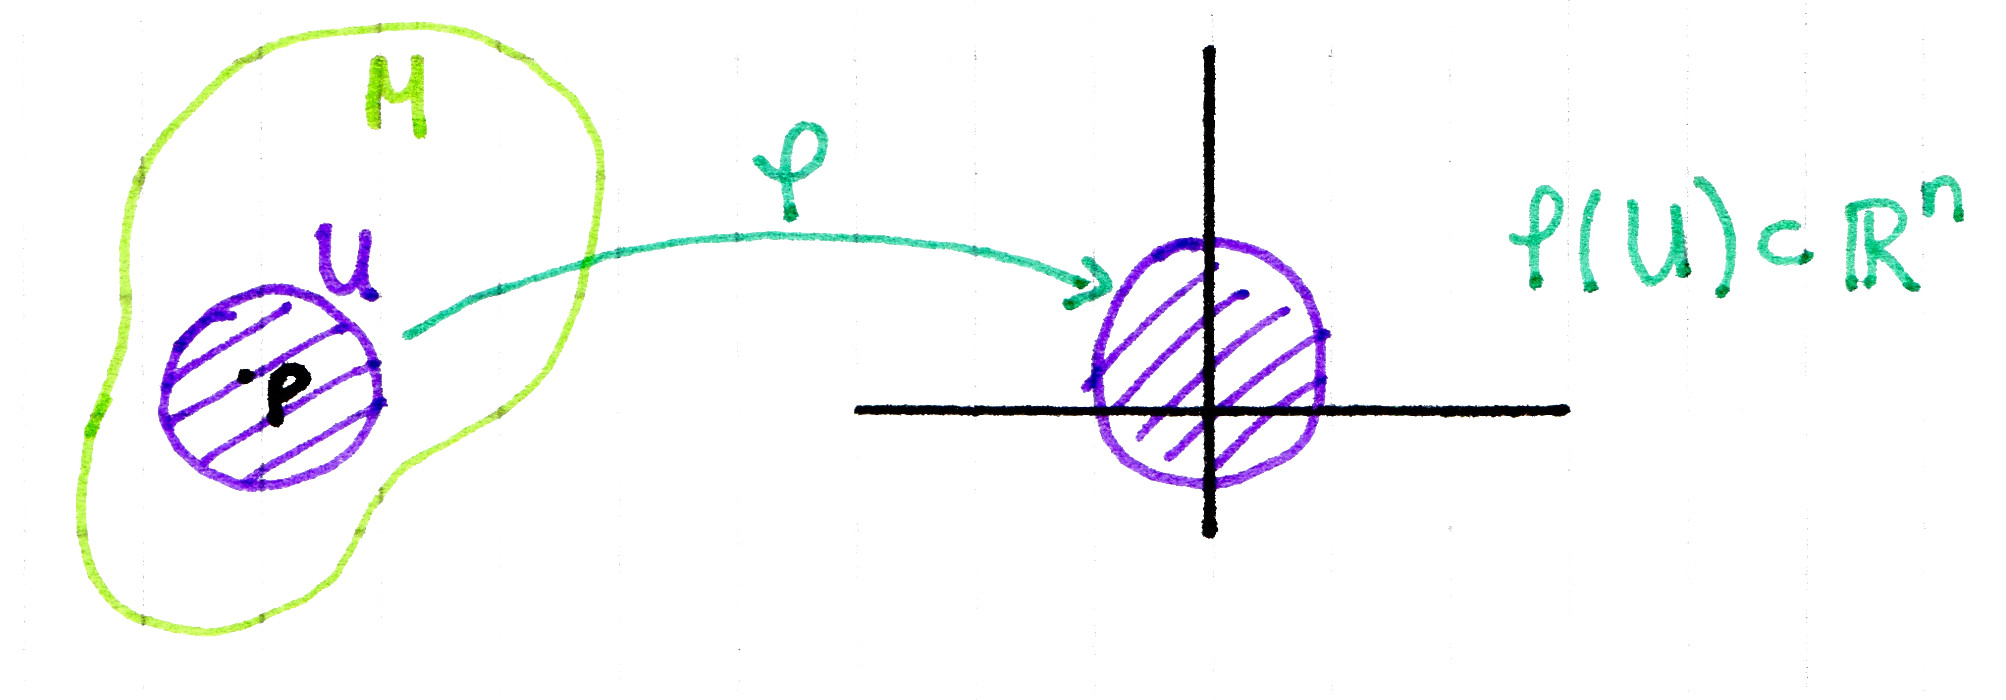
\includegraphics[width=.5\textwidth]{Karte}
      \caption{Karte von \( U \) mittels \( \phi \)}
    \end{figure}
    \item \( M \) ist \hyperref[def:hausdorffsch]{hausdorffsch} und besitzt abzählbare Basis der Topologie.
  \end{enumerate}
  \emph{Bemerkung}:
  \begin{itemize}
    \item Die zweite Eigenschaft ist ``technisch'' und garantiert, dass eine ``Zerlegung der Eins'' existiert (braucht man z.B. für die Existenz von Riemannschen Metriken). 
    \item Die Zahl \( n \) heißt \term{Dimension}\label{def:dimension} von \( M \) (eindeutig, wenn \( M \) \hyperref[def:zusammenhaengend]{zusammenhängend} ist, siehe \hyperref[th:satzGebietstreue]{Satz von Gebietstreue}). 
  \end{itemize}
\end{definition}

\begin{example}[{{\hyperref[def:topologischeMannigfaltigkeit]{Topologische Mannigfaltigkeiten}}}]
  \
  \begin{enumerate}
    \setcounter{enumi}{-1}

    \item Eine abzählbare Menge mit \hyperref[bsp:diskreteTopologie]{diskreter Topologie} (jeder Punkt ist offen) ist eine \( 0 \)-dimensionale Mannigfaltigkeit.

    \item \( S^1 \) ist eine \hyperref[def:kompakt]{kompakte}, \hyperref[def:zusammenhaengend]{zusammenhängenge} \( 1 \)-dimensionale Mannigfaltigkeit. \\
      \( \R \) ist nichtkompakte, zusammenhängende \( 1 \)-Mannigfaltigkeit.

    \begin{figure}[H]
      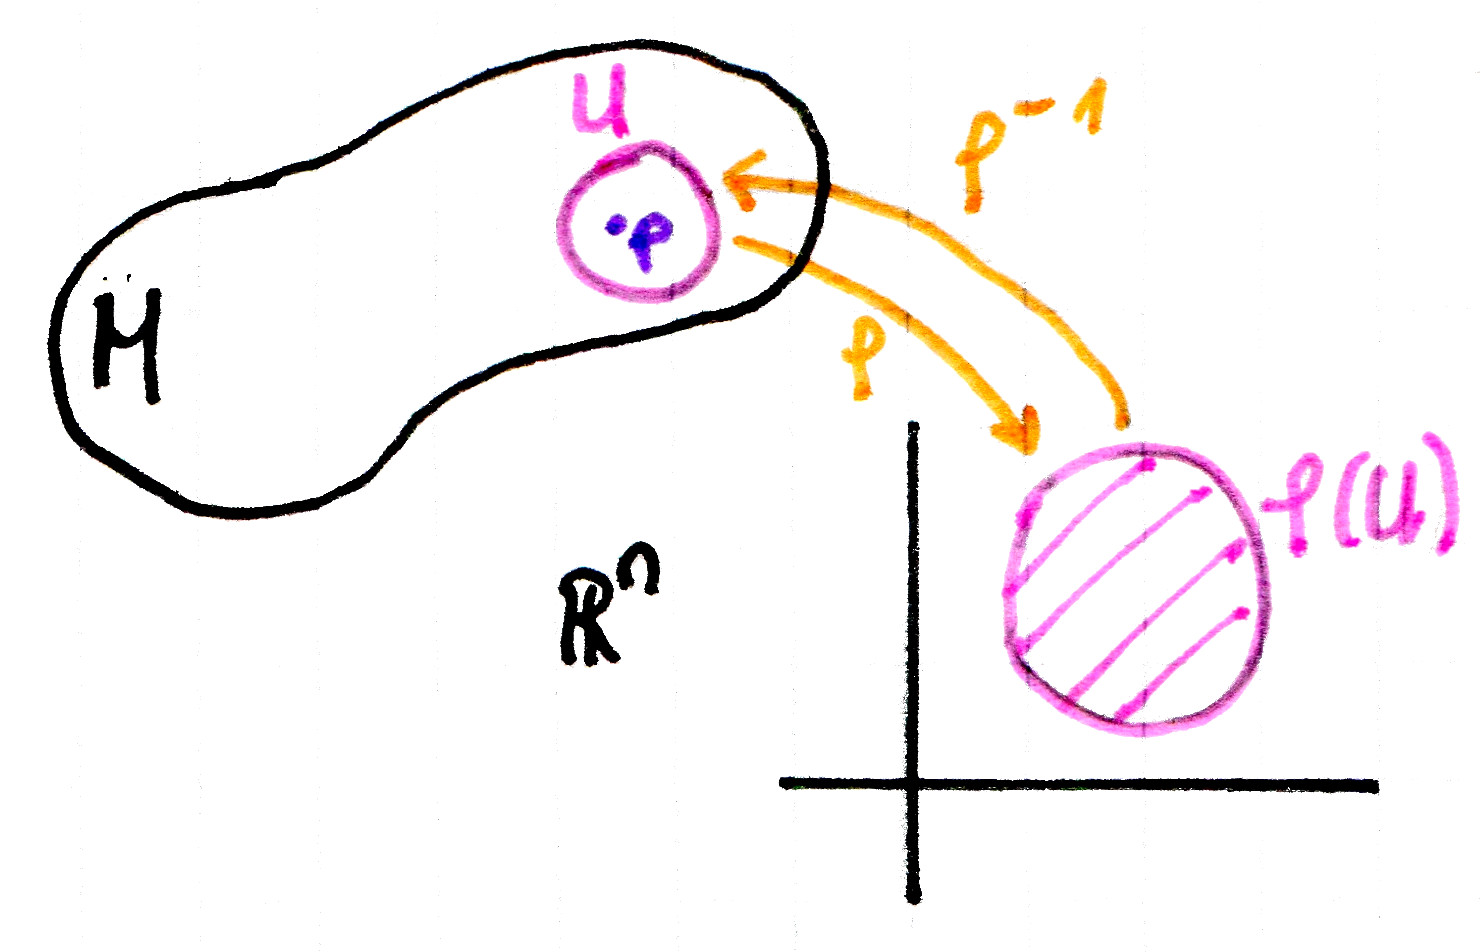
\includegraphics[width=.5\textwidth]{CharakteristikaMannigfaltigkeit}
      \captionsetup{width=.5\textwidth}
      \caption{Darstellung von \( \R \) und \( S^1 \) mit den für die topologische Mannigfaltigkeit nötigen Charakteristika}
    \end{figure}

    \item Jede offene Teilmenge einer Mannigfaltigkeit ist wieder eine Mannigfaltigkeit, z.B. ist jede offene Teilmenge von \( \R^n \) eine \( n \)-dimensionale Mannigfaltigkeit (hier ist \hyperref[def:karte]{Karte} = Einschränkung der Identität). \\
    \emph{Spezialfall}: \( \text{GL}(n,\R) = \{ A \in \R^{n \times n} : \det A \neq 0 \} \) ist offene Teilmenge von \( \R^{n^2} \), also eine \( n^2 \)-dimensionale Mannigfaltigkeit, denn:
    \begin{itemize}
      \item \( \det : \R^{n \times n} \to \R \) ist stetig
      \item \( \{ 0 \} \) ist abgeschlossen in \( \R \)
      \item \( \det^{-1} \{ 0 \} \) ist abgeschlossen in \( \R^{n \times n} \)
      \item \( \R^{n \times n} \setminus \det^{-1} \{ 0 \} = \text{GL}(n,\R ) \) ist offen in \( \R^{n \times n} \)
    \end{itemize}

    \begin{minipage}{.45\textwidth}
      \item Die \hyperref[bsp:einheitssphaere]{\( n \)-dimensionale Sphäre} mit Radius \( R > 0 \),
      \begin{equation*}
        S^n_R = \{ x \in \R^{n+1} : \Vert x \Vert = R \}\text{,}
      \end{equation*}
      ist \( n \)-dimensionale topologische Mannigfaltigkeit.
    \end{minipage}
    \hfill
    \begin{minipage}{.45\textwidth}
      \begin{figure}[H]
        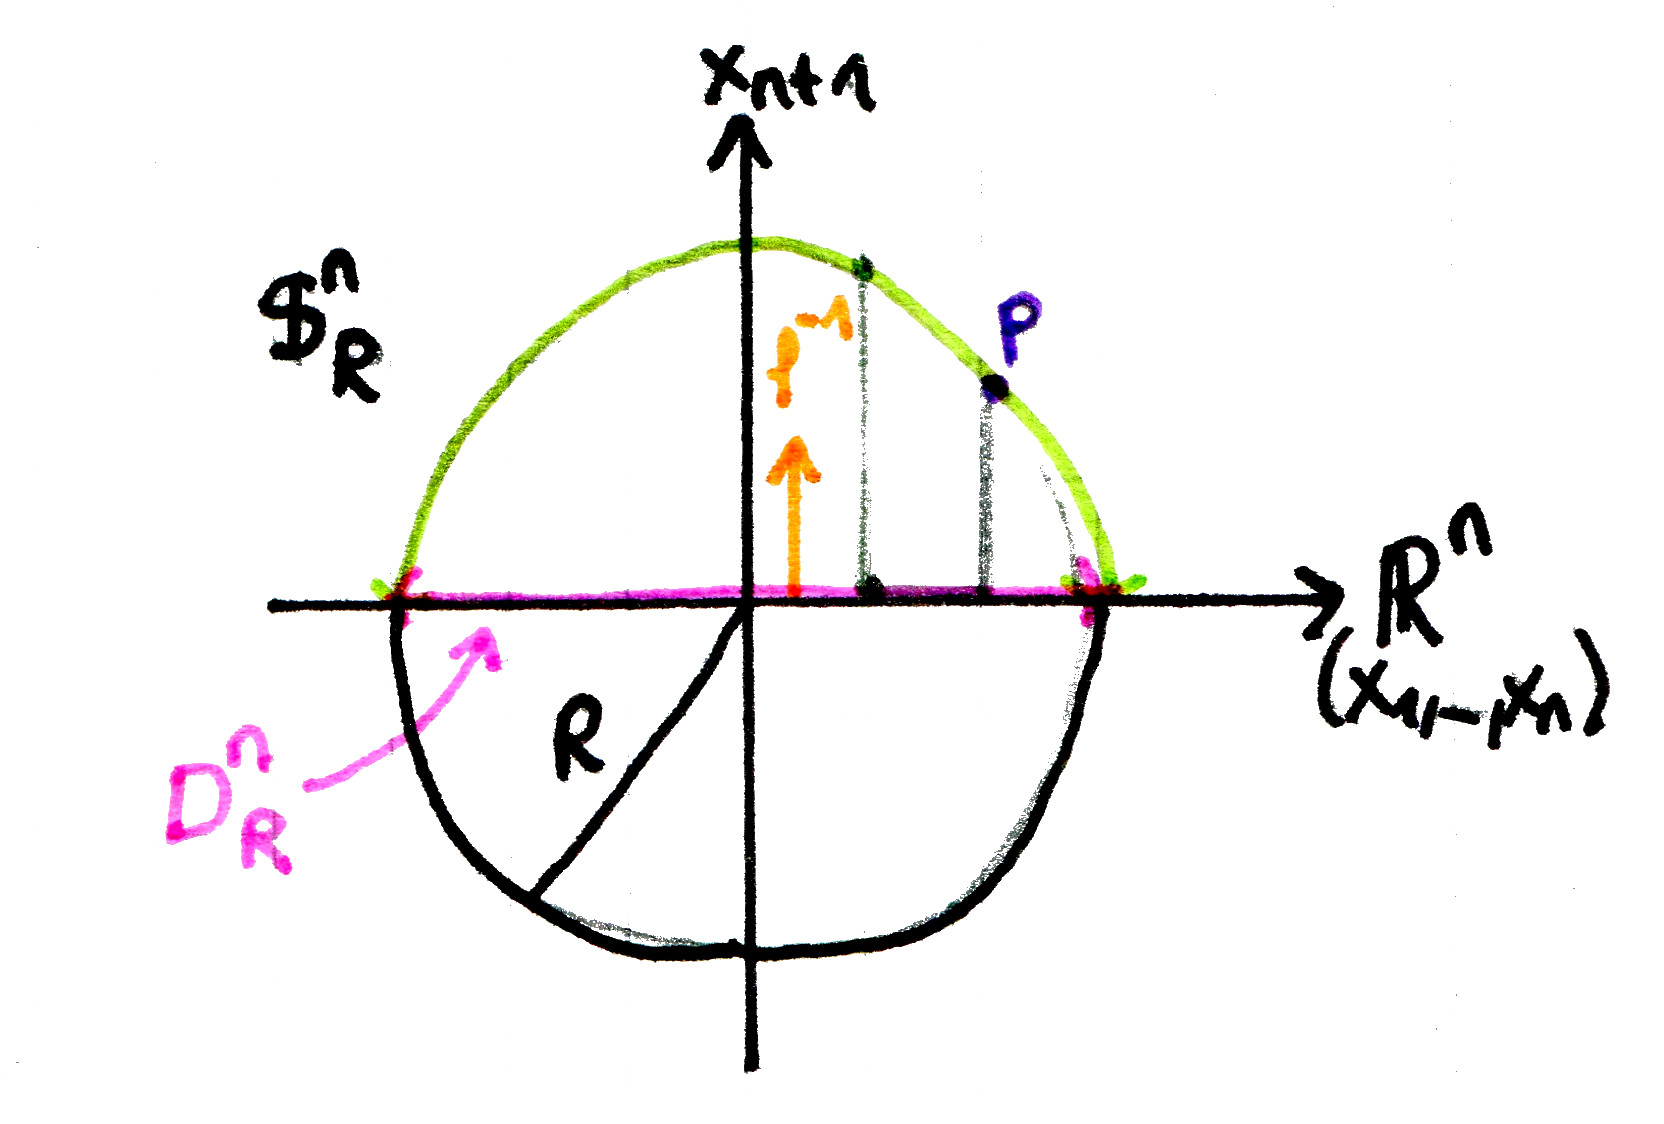
\includegraphics[width=.8\textwidth]{SphaereMannigfaltigkeit}
        \caption{\( n \)-dimensionale Sphäre als topologische Mannigfaltigkeit}
      \end{figure}
    \end{minipage}
    \begin{proof}
      Sei \( (x_1, \dots, x_{n+1}) = p \in S^n_R \), oBdA \( x_{n+1} > 0 \). Man betrachte die Abbildung
      \begin{align*}
        \phi^{-1} : D^n_R \coloneqq \left \{ x \in \R^n : \Vert x \Vert < R \right \} &\to \phi(D^n_R) \subset S^n_R \\
          (x_1, \dots, x_n) &\mapsto \left(x_1, \dots, x_n, \sqrt{R^2-(x_1^2 + \cdots + x_n^2)}\right)
      \end{align*}
      d.h. \( \phi \) ist Einschränkung der Orthogonalprojektion
      \begin{align*}
        \R^{n+1} &\to \R^n \subset \R^{n+1} \\
          (x_1, \dots, x_{n+1}) &\mapsto (x_1, \dots, x_n, 0)
      \end{align*}
      auf \( S_R^n \).
      \begin{figure}[H]
        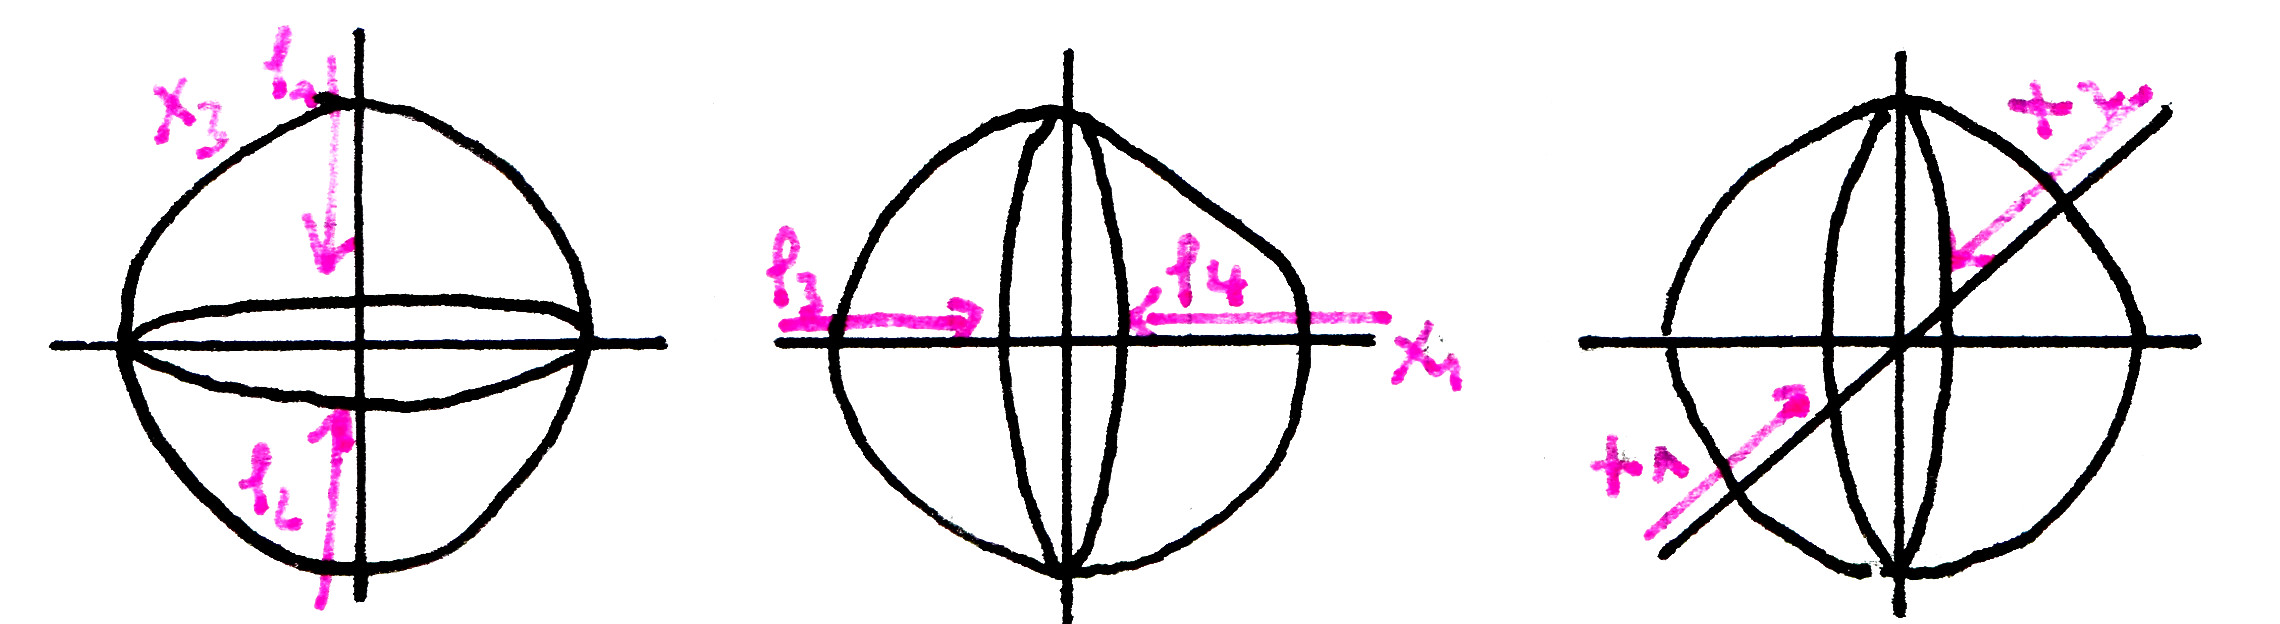
\includegraphics[width=.5\textwidth]{Orthogonalprojektion}
        \caption{Einschränkung der Orthogonalprojektion}
      \end{figure}
      Alternativ kann via stereographischer Projektion mit \( 2 \) Karten ausgekommen werden. \\
      Ein \hyperref[def:atlas]{Atlas} mit einer Karte existiert nicht. \qed{}
    \end{proof}
    \item Das Produkt von \( n_1 \)-dimensionaler Mannigfaltigkeit \( M_1 \) und \( n_2 \)-dimensionaler Mannigfaltigkeit \( M_2 \) ist \( (n_1+n_2) \)-dimensionale Mannigfaltigkeit. \\
    \emph{Karten}: \( (p_1, p_2) \in M_1 \times M_2 \),
    \begin{equation*}
      \widetilde{\phi} : U_1 \times U_2 \to \phi_1(U_1) \times \phi_2(U_2) \subset \R^{n_1} \times \R^{n_2}
    \end{equation*}
    mit \( (U_1, \phi_1) \) Karte von \( M_1 \) um \( p_1 \) und \( (U_2, \phi_2) \) Karte von \( M_2 \) um \( p_2 \).
  \end{enumerate}
\end{example}

\begin{remark}[``Wieviele {\hyperref[def:topologischeMannigfaltigkeit]{topologische Mannigfaltigkeiten}} gibt es?'']
  \
  \begin{itemize}
    \item \emph{Dimension} \( n=1 \): Im wesentlichen \( \R \) (nicht \hyperref[def:kompakt]{kompakt}) oder \( S^1 \) (kompakt).
    \item \emph{Dimension} \( n=2 \): Liste für \hyperref[def:zusammenhaengend]{zusammenhängende}, kompakte, ``orientierbare'', ``randlose'' Mannigfaltigkeiten:
    \begin{itemize}
      \item \( g = 0 \): \( S^2 \) \hyperref[bsp:einheitssphaere]{Einheitssphäre}
      \item \( g = 1 \): \( T^2 = S^1 \times S^1 \) Torus
      \item \( g = 2 \): Brezel
      \item \dots 
    \end{itemize}
    \( g \) ist das \term{Geschlecht}\label{def:geschlecht} der Mannigfaltigkeit.
    \item \emph{Dimension} \( n=3 \): Thurston's \term{Geometrisierungs-Vermutung}\label{theorem:geometrisierungsvermutung} (\( \sim \) 1978) \\
      Bewiesen von Perelman (2002), ein Milleniumsproblem.
    \item \emph{Dimension} \( n \geq 4 \): Allgemeine Klassifikation unmöglich, weil das Homöomorphieproblem hier nicht entscheidbar ist (Markov, 1960).
  \end{itemize}
\end{remark}

\section{Differenzierbare Mannigfaltigkeiten}

\begin{definition}[Kartenwechsel, differenzierbare Mannigfaltigkeit]
  \  \\

  \begin{minipage}{.45\textwidth}
    Sei \( M \) \hyperref[def:topologischeMannigfaltigkeit]{topologische Mannigfaltigkeit}, \( p \in M \). Ein \term{Kartenwechsel}\label{def:kartenwechsel} ist ein \hyperref[def:homoeomorphismus]{Homöomorphismus}
    \begin{equation*}
      \psi \circ \phi^{-1}: \underbrace{\phi(D)}_{\subset \R^n} \to \underbrace{\psi(D)}_{\subset \R^n}\text{.}
    \end{equation*}
  \end{minipage}
  \hfill
  \begin{minipage}{.45\textwidth}
    \begin{figure}[H]
      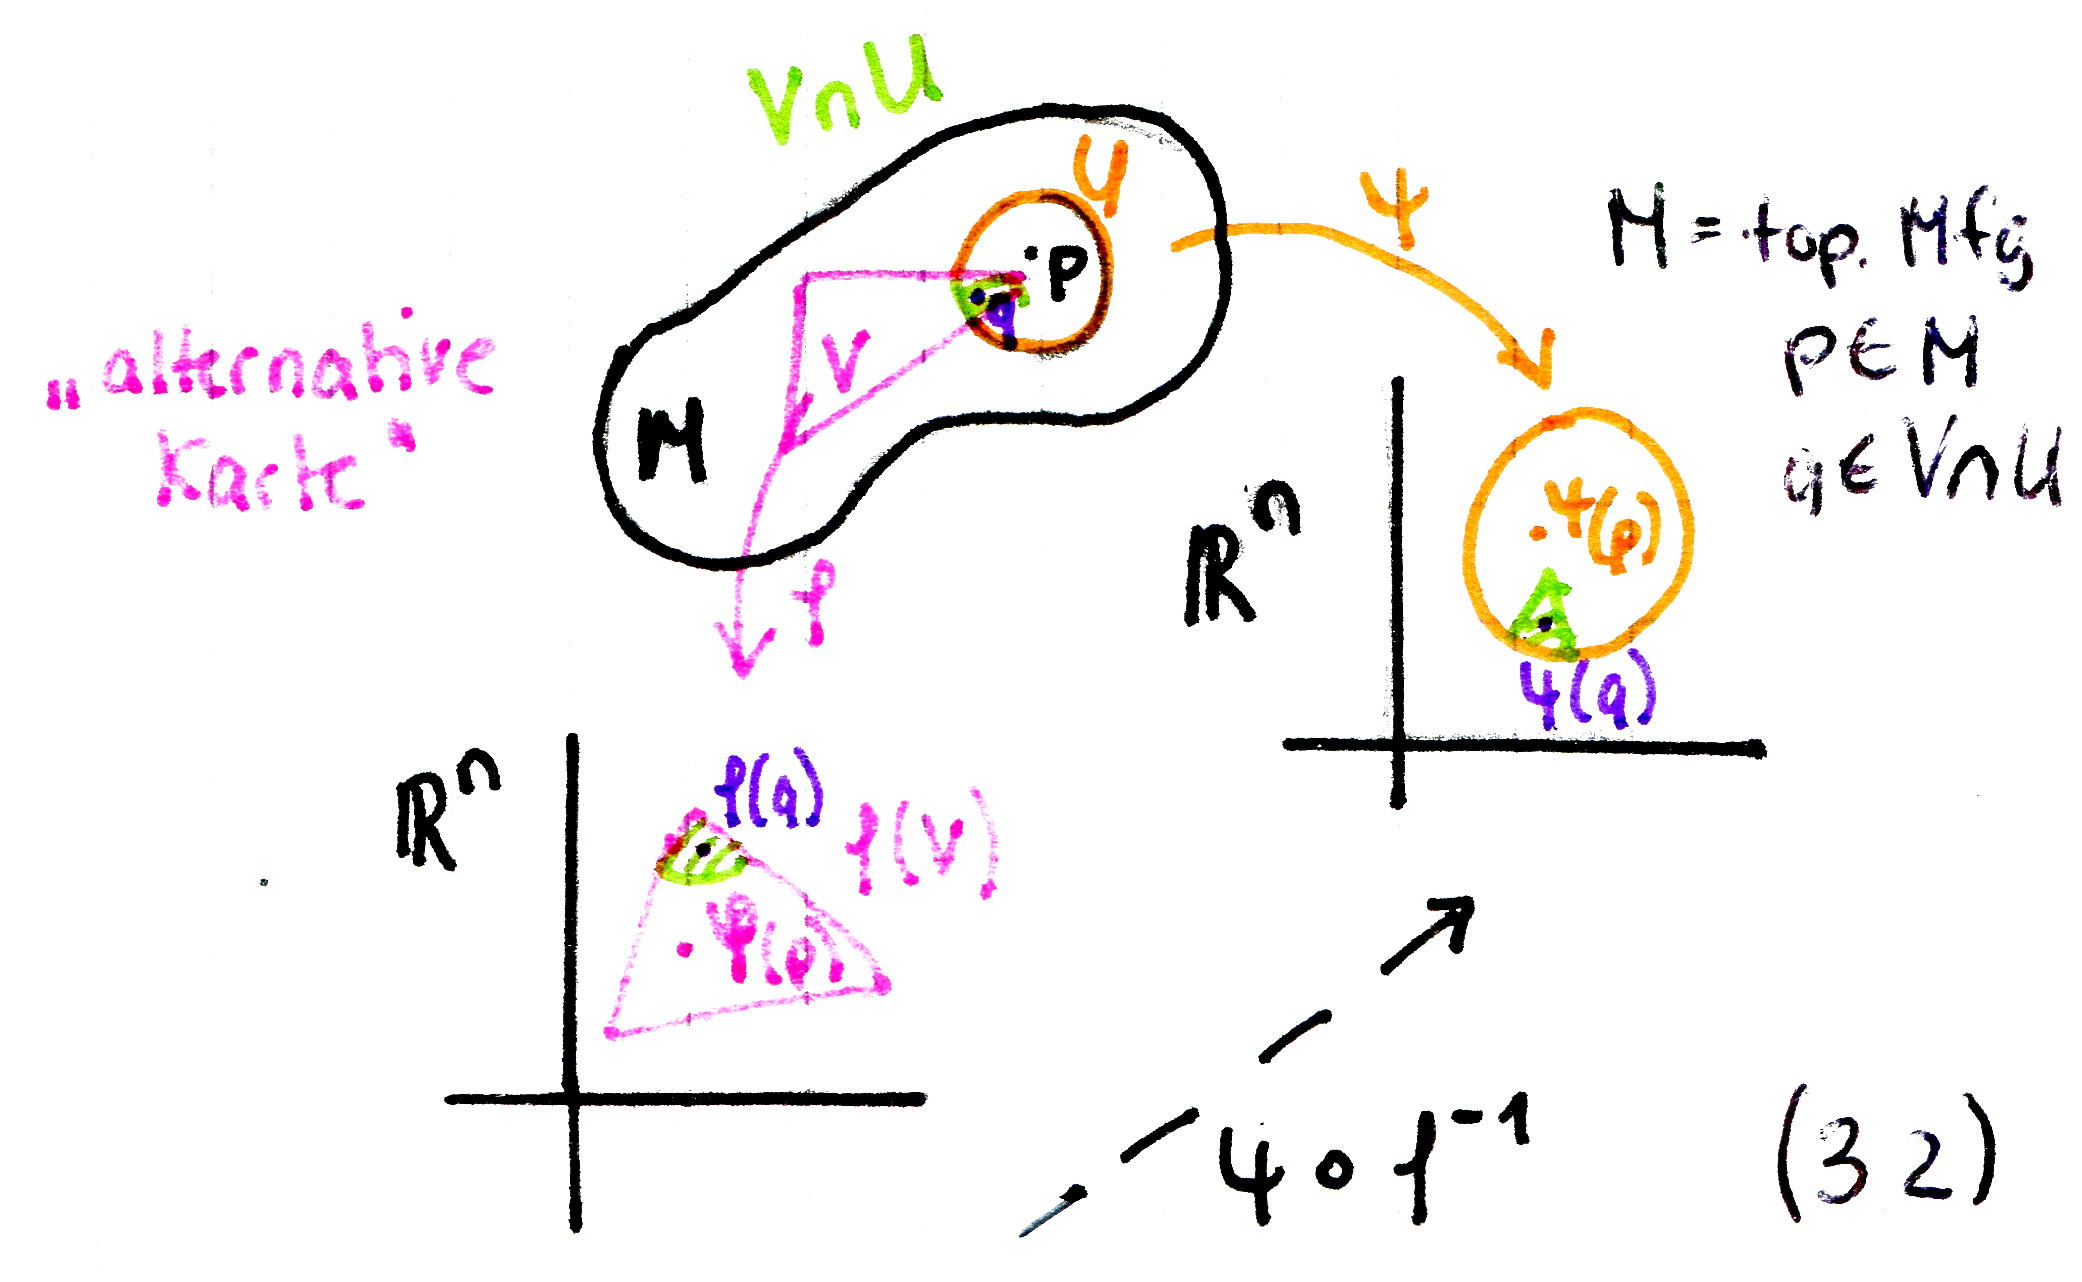
\includegraphics[width=\textwidth]{Kartenwechsel}
      \caption{Kartenwechsel}
    \end{figure}
  \end{minipage}
  Ein \hyperref[def:atlas]{Atlas} \( \mathcal{A} \) von \( M \) ist ein \term{\( C^\infty \)-Atlas}\label{def:dbatlas}, falls alle möglichen Kartenwechsel \( C^\infty \)-Abbildungen von \( \R^n \) sind, also alle partiellen Ableitungen existieren und stetig sind. \\
  Ein maximaler \( C^\infty \)-Atlas heißt \term{\( C^\infty \)-Struktur}\label{def:dbstruktur} auf der topologischen Mannigfaltigkeit \( M \). Eine \( C^\infty \)-Mannigfaltigkeit ist eine topologische Mannigfaltigkeit mit einer \( C^\infty \)-Struktur (auch \term{glatte}\label{def:glattemannigfaltigkeit} oder \term{differenzierbare Mannigfaltigkeit}\label{def:dbmannigfaltigkeit}).
\end{definition}

\begin{remark}
  \
  \begin{enumerate}
    \item Es gibt \hyperref[def:topologischeMannigfaltigkeit]{topologische Mannigfaltigkeiten} ohne \hyperref[def:dbstruktur]{differenzierbare Struktur}\footnote{Kerraire 1960}.
    \item Auf \( \R^n \), \( n \neq 4 \)\footnote{Kirby, Friedman 1980}, existiert genau eine differenzierbare Struktur.
    \item Auf \( S^7 \) existieren \( 28 \) differenzierbare Strukturen\footnote{Milnor 1956}.
  \end{enumerate}
  \emph{Frage}: Wozu das Differenzierbarkeitskriterium für \hyperref[def:kartenwechsel]{Kartenwechsel}? Beispielsweise für die Definition von differenzierbaren Abbildungen zwischen \hyperref[def:dbmannigfaltigkeit]{differenzierbaren Mannigfaltigkeiten}.
\end{remark}


\begin{definition}[Differenzierbarkeit]
  Seien \( M^m \), \( N^n \) \hyperref[def:dbmannigfaltigkeit]{differenzierbare Mannigfaltigkeiten} und \( F: M^m \to N^n \) stetig. \( F \) heißt \term{differenzierbar in \( p \in M \)}\label{def:differenzierbar}, falls für \hyperref[def:karte]{Karten} \( (U, \phi) \) um \( p \) und \( (V, \psi) \) um \( F(p) \) gilt:
  \begin{equation*}
    \psi \circ F \circ \phi^{-1}: \underbrace{\phi(U)}_{\subset \R^m} \to \underbrace{\psi(V)}_{\subset \R^n}
  \end{equation*}
  ist \( C^\infty \)-Abbildung in \( \phi(p) \). \\
  So kommt man von einem abstrakten \( F \) zwischen den Mannigfaltigkeiten zu einer konkreten Darstellung von \( F \). \\
  \( F \) heißt \term{differenzierbar} (\( C^\infty \)), falls \( F \) differenzierbar ist für alle \( p \in M \).
  \begin{figure}[H]
    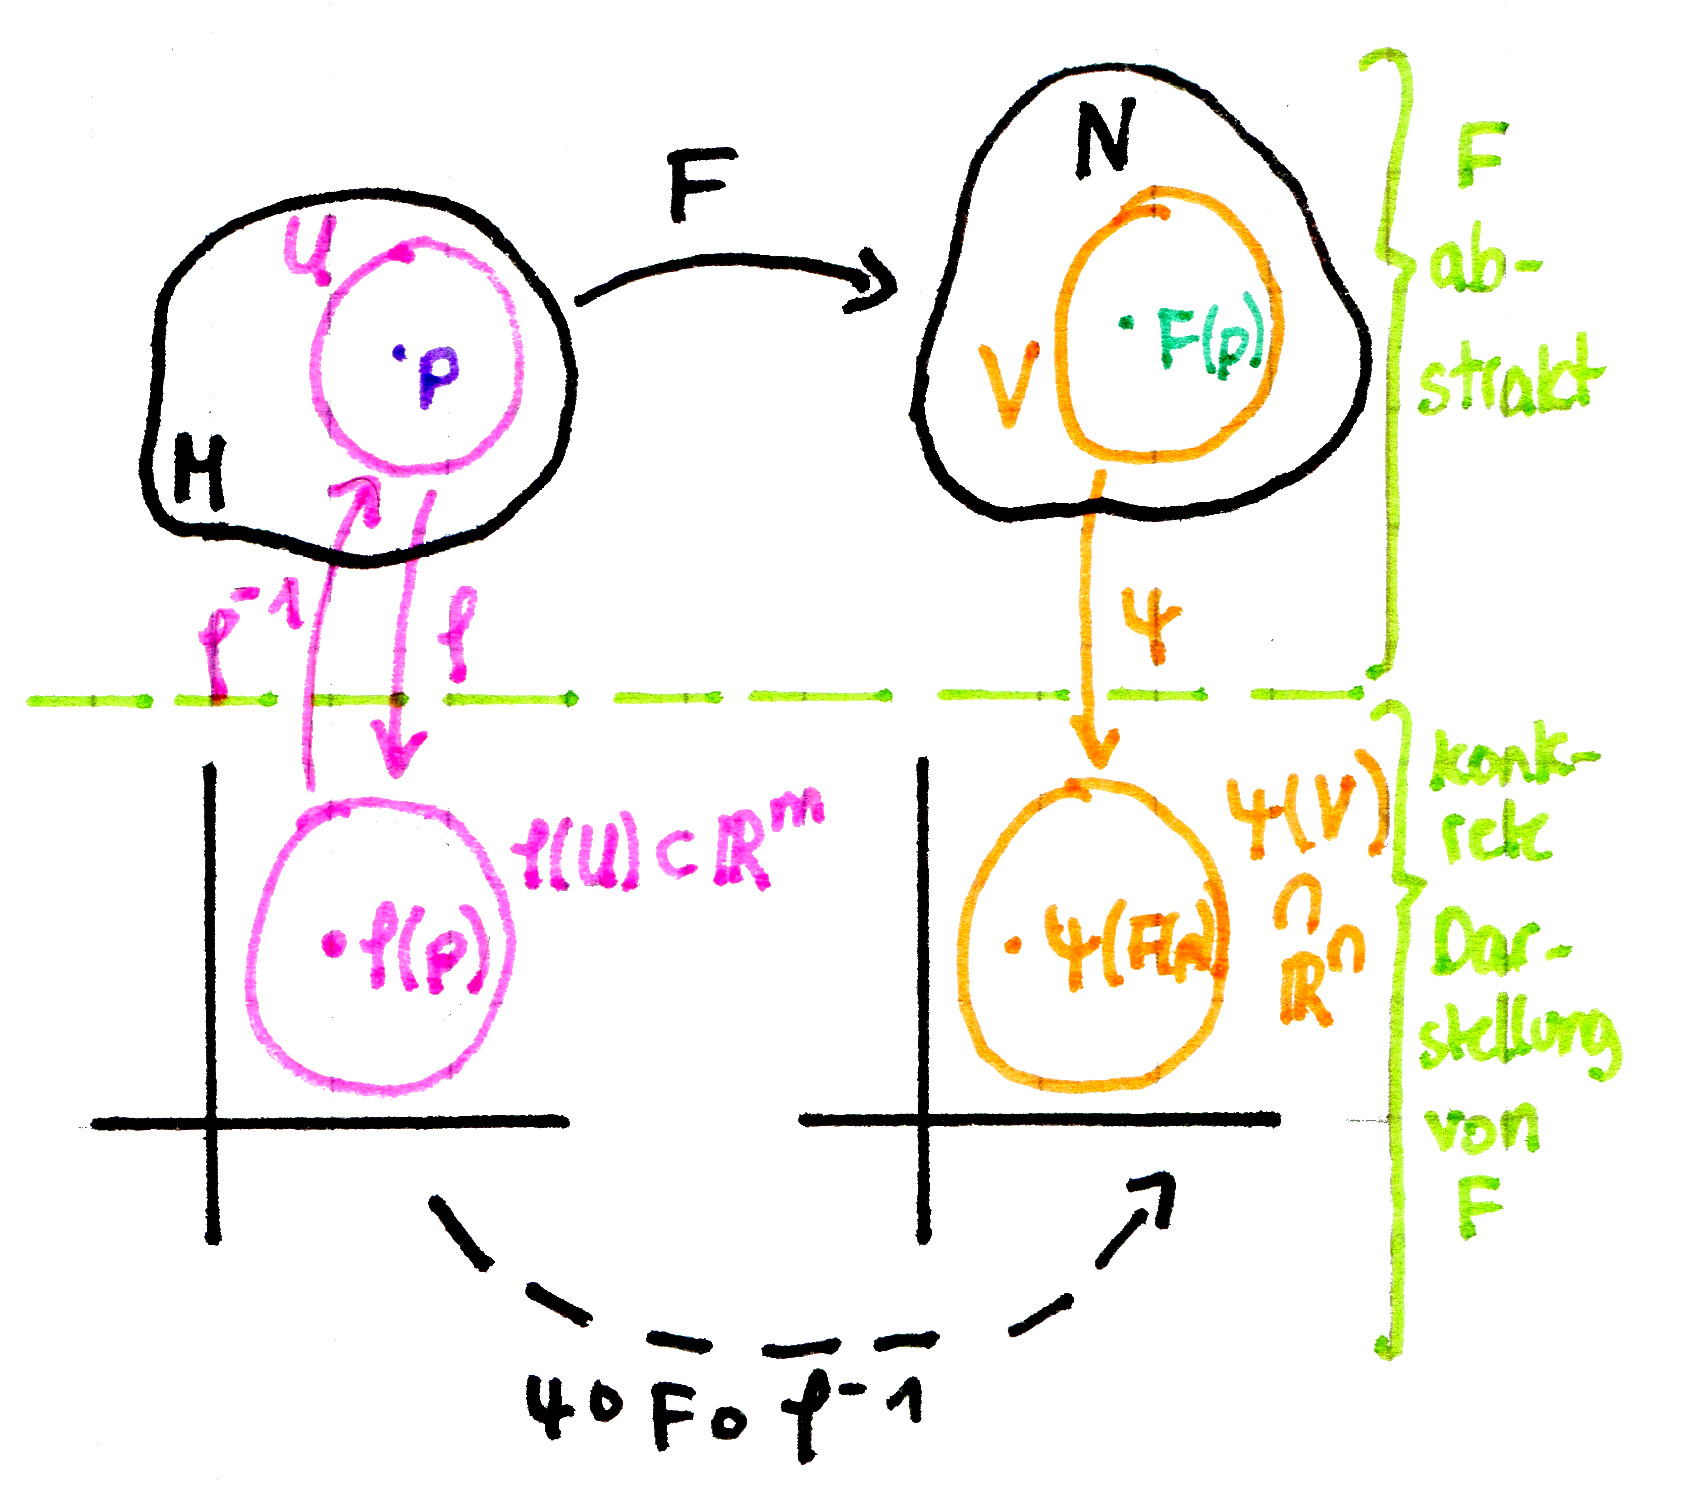
\includegraphics[width=.5\textwidth]{Differenzierbarkeitskriterium}
    \caption{Differenzierbarkeitskriterium}
  \end{figure}
\end{definition}

\begin{remark}[Wohldefiniertheit der Differenzierbarkeit]
  Differenzierbarkeit in \( p \) ist wohldefiniert (also unabhängig von der Wahl der Karten)
  \begin{proof}
    \emph{Erster Test}: \( \psi \circ F \circ \phi^{-1} \), \emph{zweiter Test} \( \widetilde{\psi} \circ F \circ \widetilde{\phi}^{-1} \) \\
    Es gilt:
    \begin{align*}
      \psi \circ F \circ \phi^{-1} &= \psi \circ \underbrace{\widetilde{\psi}^{-1} \circ \widetilde{\psi}}_{\text{Id}_{\R^n}} \circ F \circ \underbrace{\widetilde{\phi}^{-1} \circ \widetilde{\phi}}_{\text{Id}_{\R^n}} \circ \phi^{-1} \\
        &= \underbrace{\left( \psi \circ \widetilde{\psi}^{-1} \right)}_{C^\infty} \circ \left( \widetilde{\psi} \circ F \circ \widetilde{\phi}^{-1} \right) \circ \underbrace{\left( \widetilde{\phi} \circ \phi^{-1} \right)}_{\text{Kartenwechsel}}
    \end{align*}
    Also: Abbildung in Test 1 ist \( C^\infty \Leftrightarrow \) Abbildung in Test 2 ist \( C^\infty \). \qed{}
  \end{proof}
\end{remark}

\begin{remark}
  \
  \begin{itemize}
    \item \( N = \R \), \( F:M \to \R \) (differenzierbar) heißt \term{differenzierbare Funktion}.
    \item \( M = \R \) (oder \( I \subset \R \)), \( F: I \to N \) heißt \term{differenzierbare Kuve}.
    \item Eine Abbildung \( F: M \to N \) zwischen differenzierbaren Mannigfaltigkeiten heißt \term{Diffeomorphismus}\label{def:diffeomorphismus}, falls \( F \) bijektiv und \( F \) und \( F^{-1} \) differenzierbar sind (also \( C^\infty \)).
    \item Ein Homöomorphismus ist nicht unbedingt ein Diffeomorphismus. Beispielsweise \( \R \) mit Id als Karte, \( F : \R \to \R \), \( x \mapsto x^3 \) ist Homöomorphismus, aber kein Diffeomorphismus, da \( F^{-1} : x \mapsto \sqrt[3]{x} \) ist nicht \( C^\infty \).
    \item Die Menge der Diffeomorphismen einer differenzierbaren Mannigfaltigkeit ist eine Gruppe mit der Verkettung von Abbildungen.
  \end{itemize}
\end{remark}

\begin{example}
  \
  \begin{enumerate}
    \item \( U \subseteq \R^n \) offen (bzgl. Standard-Topologie). \\
      \( \phi_0 \coloneqq \text{Id}\mid_U \) mit zugehörigem maximalen Atlas definiert \( C^\infty \)-Struktur auf \( U \), die kanonische differenzierbare Struktur.
    \item \( 2 \)-dimensionale Mannigfaltigkeiten heißen auch \term{Flächen}\label{def:flaeche}, speziell \emph{regulär parametrisierte Flächen}\footnote{Gegenstand der klassischen Differentialgeometrie, siehe auch Kapitel 5}.
  \end{enumerate}
\end{example}

\begin{definition}[Reguläre Fläche]
  Eine Teilmenge \( S \) von \( \R^3 \) (mit Teilraum-Topologie von \( \R^3 \)) heißt \term{reguläre Fläche}\label{def:regulaereFlaeche}, falls für jeden Punkt \( p \in S \) eine Umgebung \( V \) von \( p \) in \( \R^3 \) und eine Abbildung
  \begin{align*}
    F : \underset{\text{offen}}{U} \subset \R^2 &\to \underset{\text{offene TM von S}}{V \cap S} \subset \R^3 \\
      (u,v) &\mapsto (x(u,v),y(u,v),z(u,v))
  \end{align*}
  existiert, so dass gilt:
  % TODO Abbildung 2
  \begin{enumerate}
    \item \( F \) ist ein differenzierbar Homöomorphismus
    \item das Differential (Jacobi-Matrix) von \( F \),
    \begin{equation*}
       \text{d}F_q : \R^2 \supseteq T_q U \to T_{F(q)}\R^3 \cong \R^3
     \end{equation*} 
     ist \emph{injektiv} (d.h. Jacobi-Matrix hat Rang \( 2 \)) für \( \forall q \in U \).
  \end{enumerate}
  \( F \) heißt \term{lokale Parametrisierung}\label{def:lokaleParametrisierung} von \( S \).
  \begin{figure}[H]
    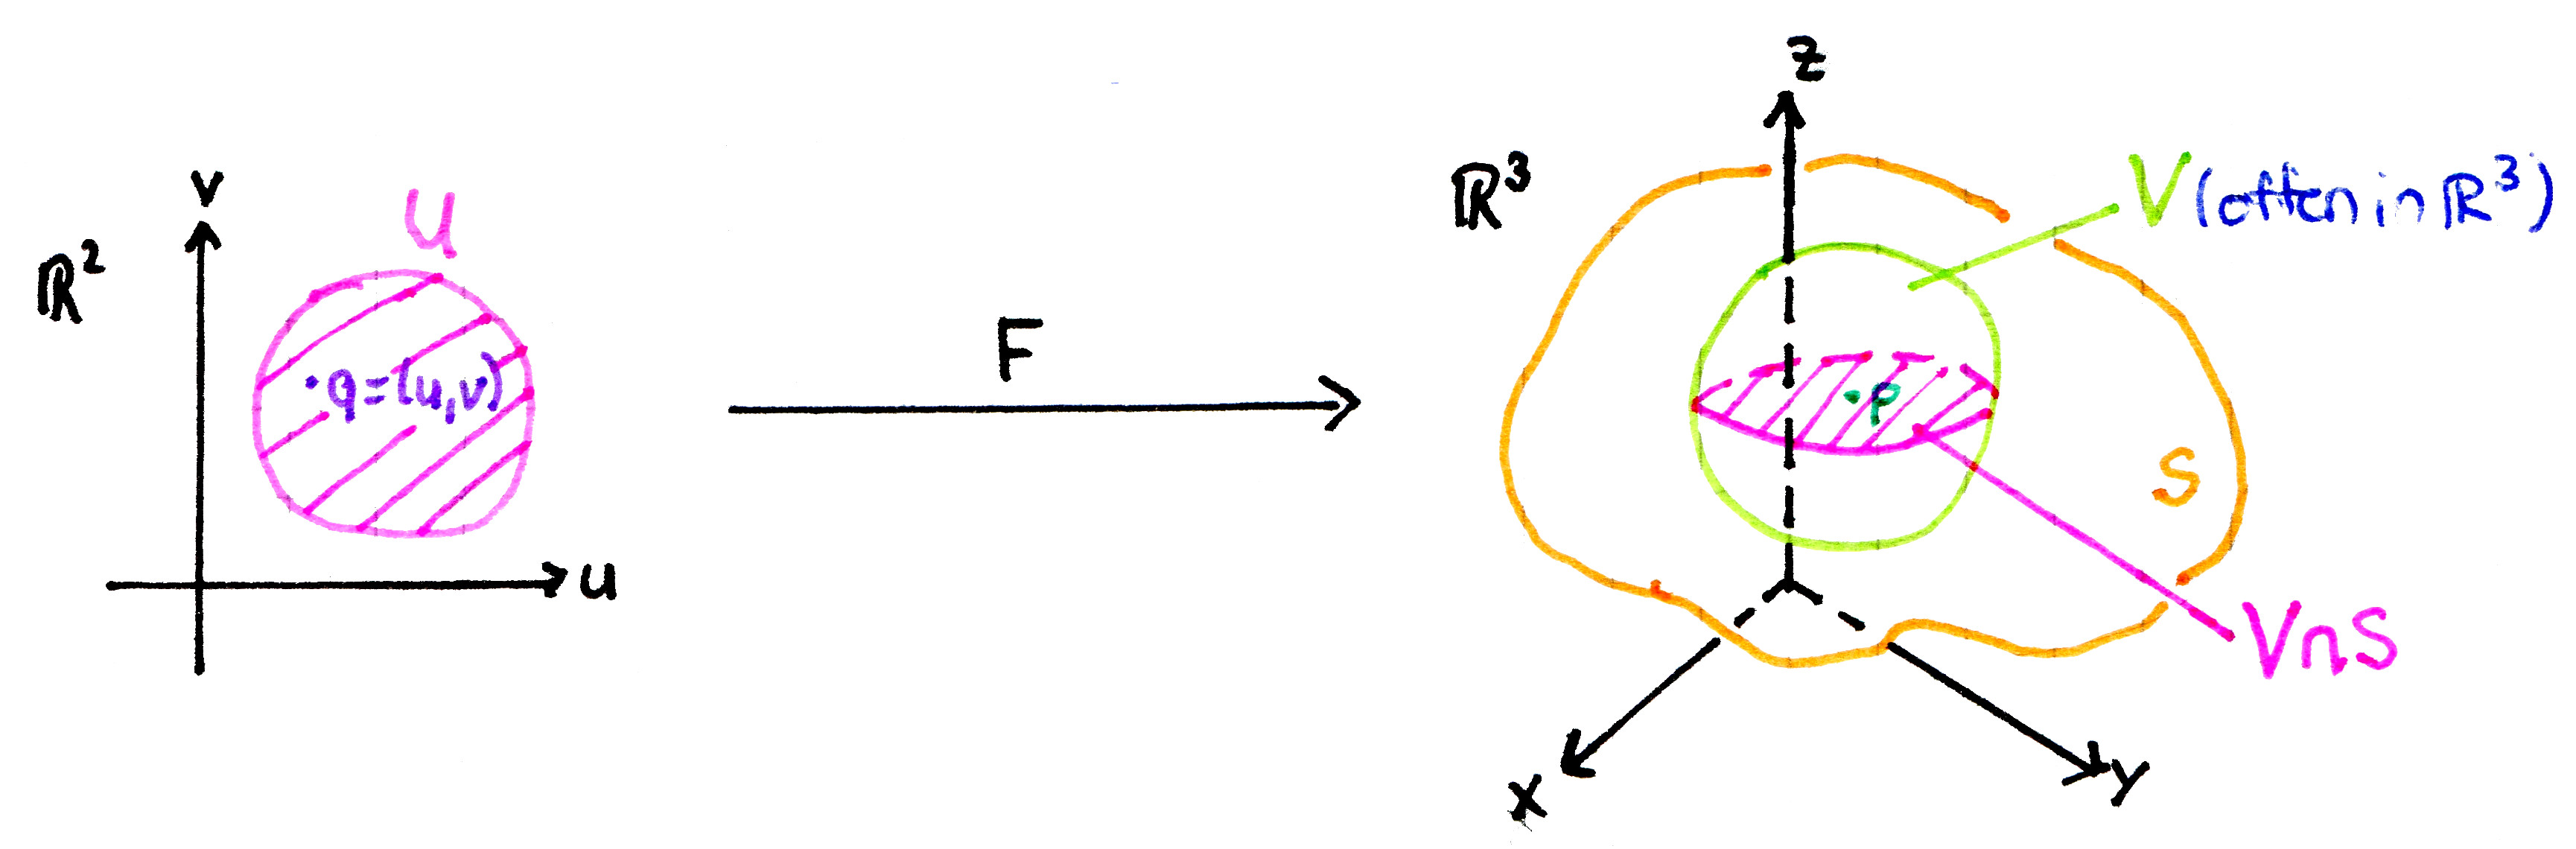
\includegraphics[width=.8\textwidth]{LokaleParametrisierung}
    \caption{Lokale Parametrisierung}
  \end{figure}
\end{definition}

\begin{example}[Rotationsfläche]
  Gegeben ist eine ebene Kurve \( c(v) = \left( r(v), 0, h(v) \right) \), \( v \in [a,b] \) mit \( r(v) > 0 \), \( c'(v) = \left( r'(v), 0, h'(v) \right) \) Tangentialvektor (mit \( C^\infty \)-Funktionen \( r \), \( h \)).\footnote{\( \Vert c'(v) \Vert \neq 0 \Leftrightarrow {(r')}^2 + {(h')}^2 \neq 0 \)}

  \begin{minipage}{.45\textwidth}
    \begin{equation*}
      F(u,v) \coloneqq \begin{pmatrix}
        r(v)\cos u \\
        r(v)\sin u \\
        h(v)
      \end{pmatrix}
    \end{equation*}
    ist reguläre Fläche.\footnotemark{} \\
    \emph{Beispiel}: \( 2 \)-Sphäre von Radius \( R \):
    \begin{equation*}
      (u,v) \mapsto \begin{pmatrix}
        R\cos v \cos u \\
        R\cos v\sin u \\
        R\sin v
      \end{pmatrix}\text{.}
    \end{equation*}
  \end{minipage}
  \footnotetext{Übung!}
  \hfill
  \begin{minipage}{.45\textwidth}
    \begin{figure}[H]
      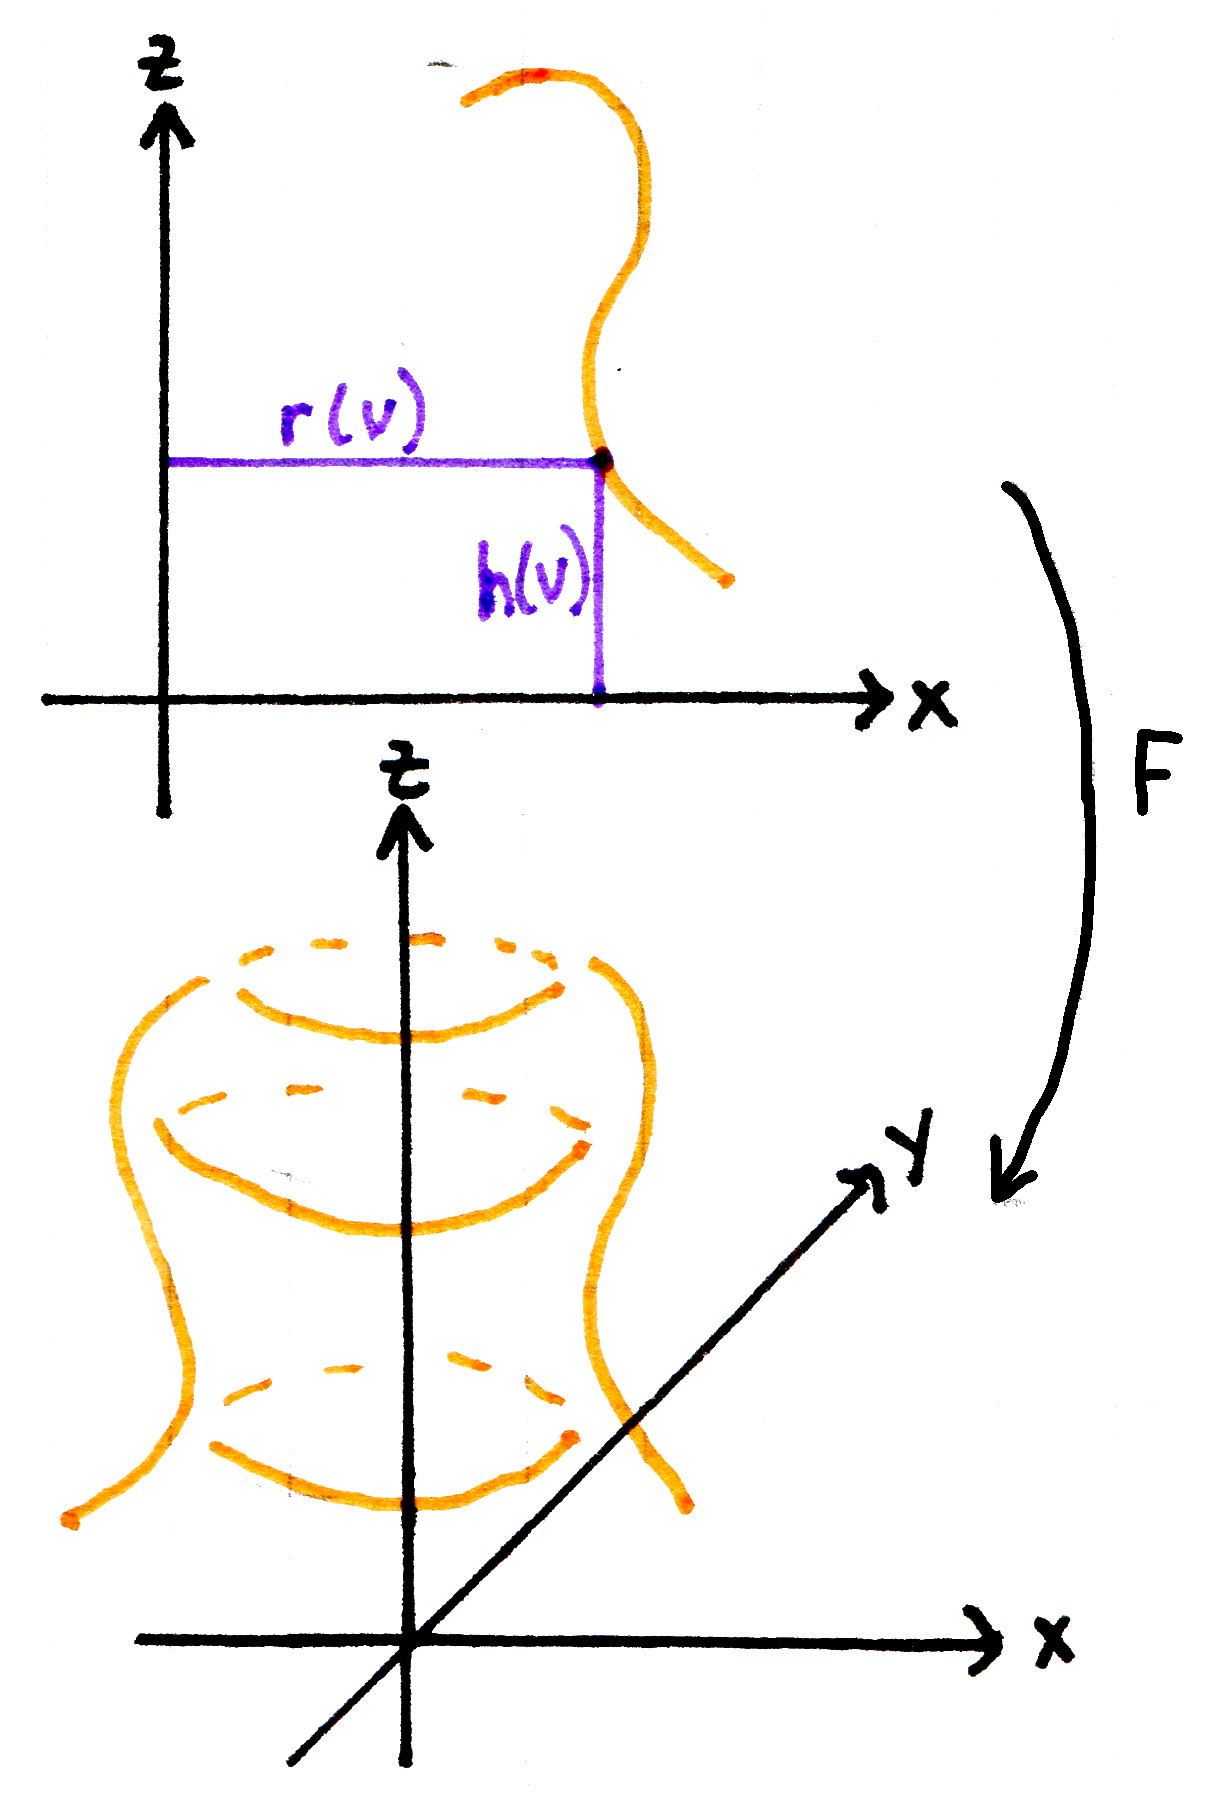
\includegraphics[width=.8\textwidth]{Rotationsflaeche}
      \caption{Rotationsfläche}
    \end{figure}
  \end{minipage}

  Es gibt andere Parametrisierungen, beispielsweise
  \begin{equation*}
    (u,v) \mapsto \begin{pmatrix}
      u \\ v \\ \sqrt{R^2-u^2-v^2}
    \end{pmatrix}
  \end{equation*}
  % TODO Abbildung 4
\end{example}

\begin{remark}[Geometrische Eigenschaften parametrisierungsunabhängig]
  \  \\
  Geometrische Eigenschaften sollten unabhängig sein von Parametrisierung. Das wird durch Eigenschaft 2 von regulären Flächen garantiert. Genauer gilt: Parameterwechsel sind differenzierbar (\( \leadsto \) reguläre Flächen sind differenzierbare \( 2 \)-dimensionale Mannigfaltigkeiten mit \( F^{-1} \) (Umkehr-Abbildung der Parametrisierung) als Karten): \\
  Sei \( p \in S \) und \( F_1 : \R^2 \supseteq U \to S \), \( F_2: \R^2 \supseteq V \to S \) zwei Parametrisierungen, sodass \( p \in F_1(U) \cap F_2(V) \eqqcolon W \). \\
  \emph{Behauptung}: Der Parameterwechsel 
  \begin{equation*}
    H \coloneqq F_1^{-1} \circ F_2 : \R^2 \supset F_2^{-1}(W) \to F_1^{-1}(W) \subset \R^2
  \end{equation*}
  ist Diffeomorphismus.
  \begin{figure}[H]
    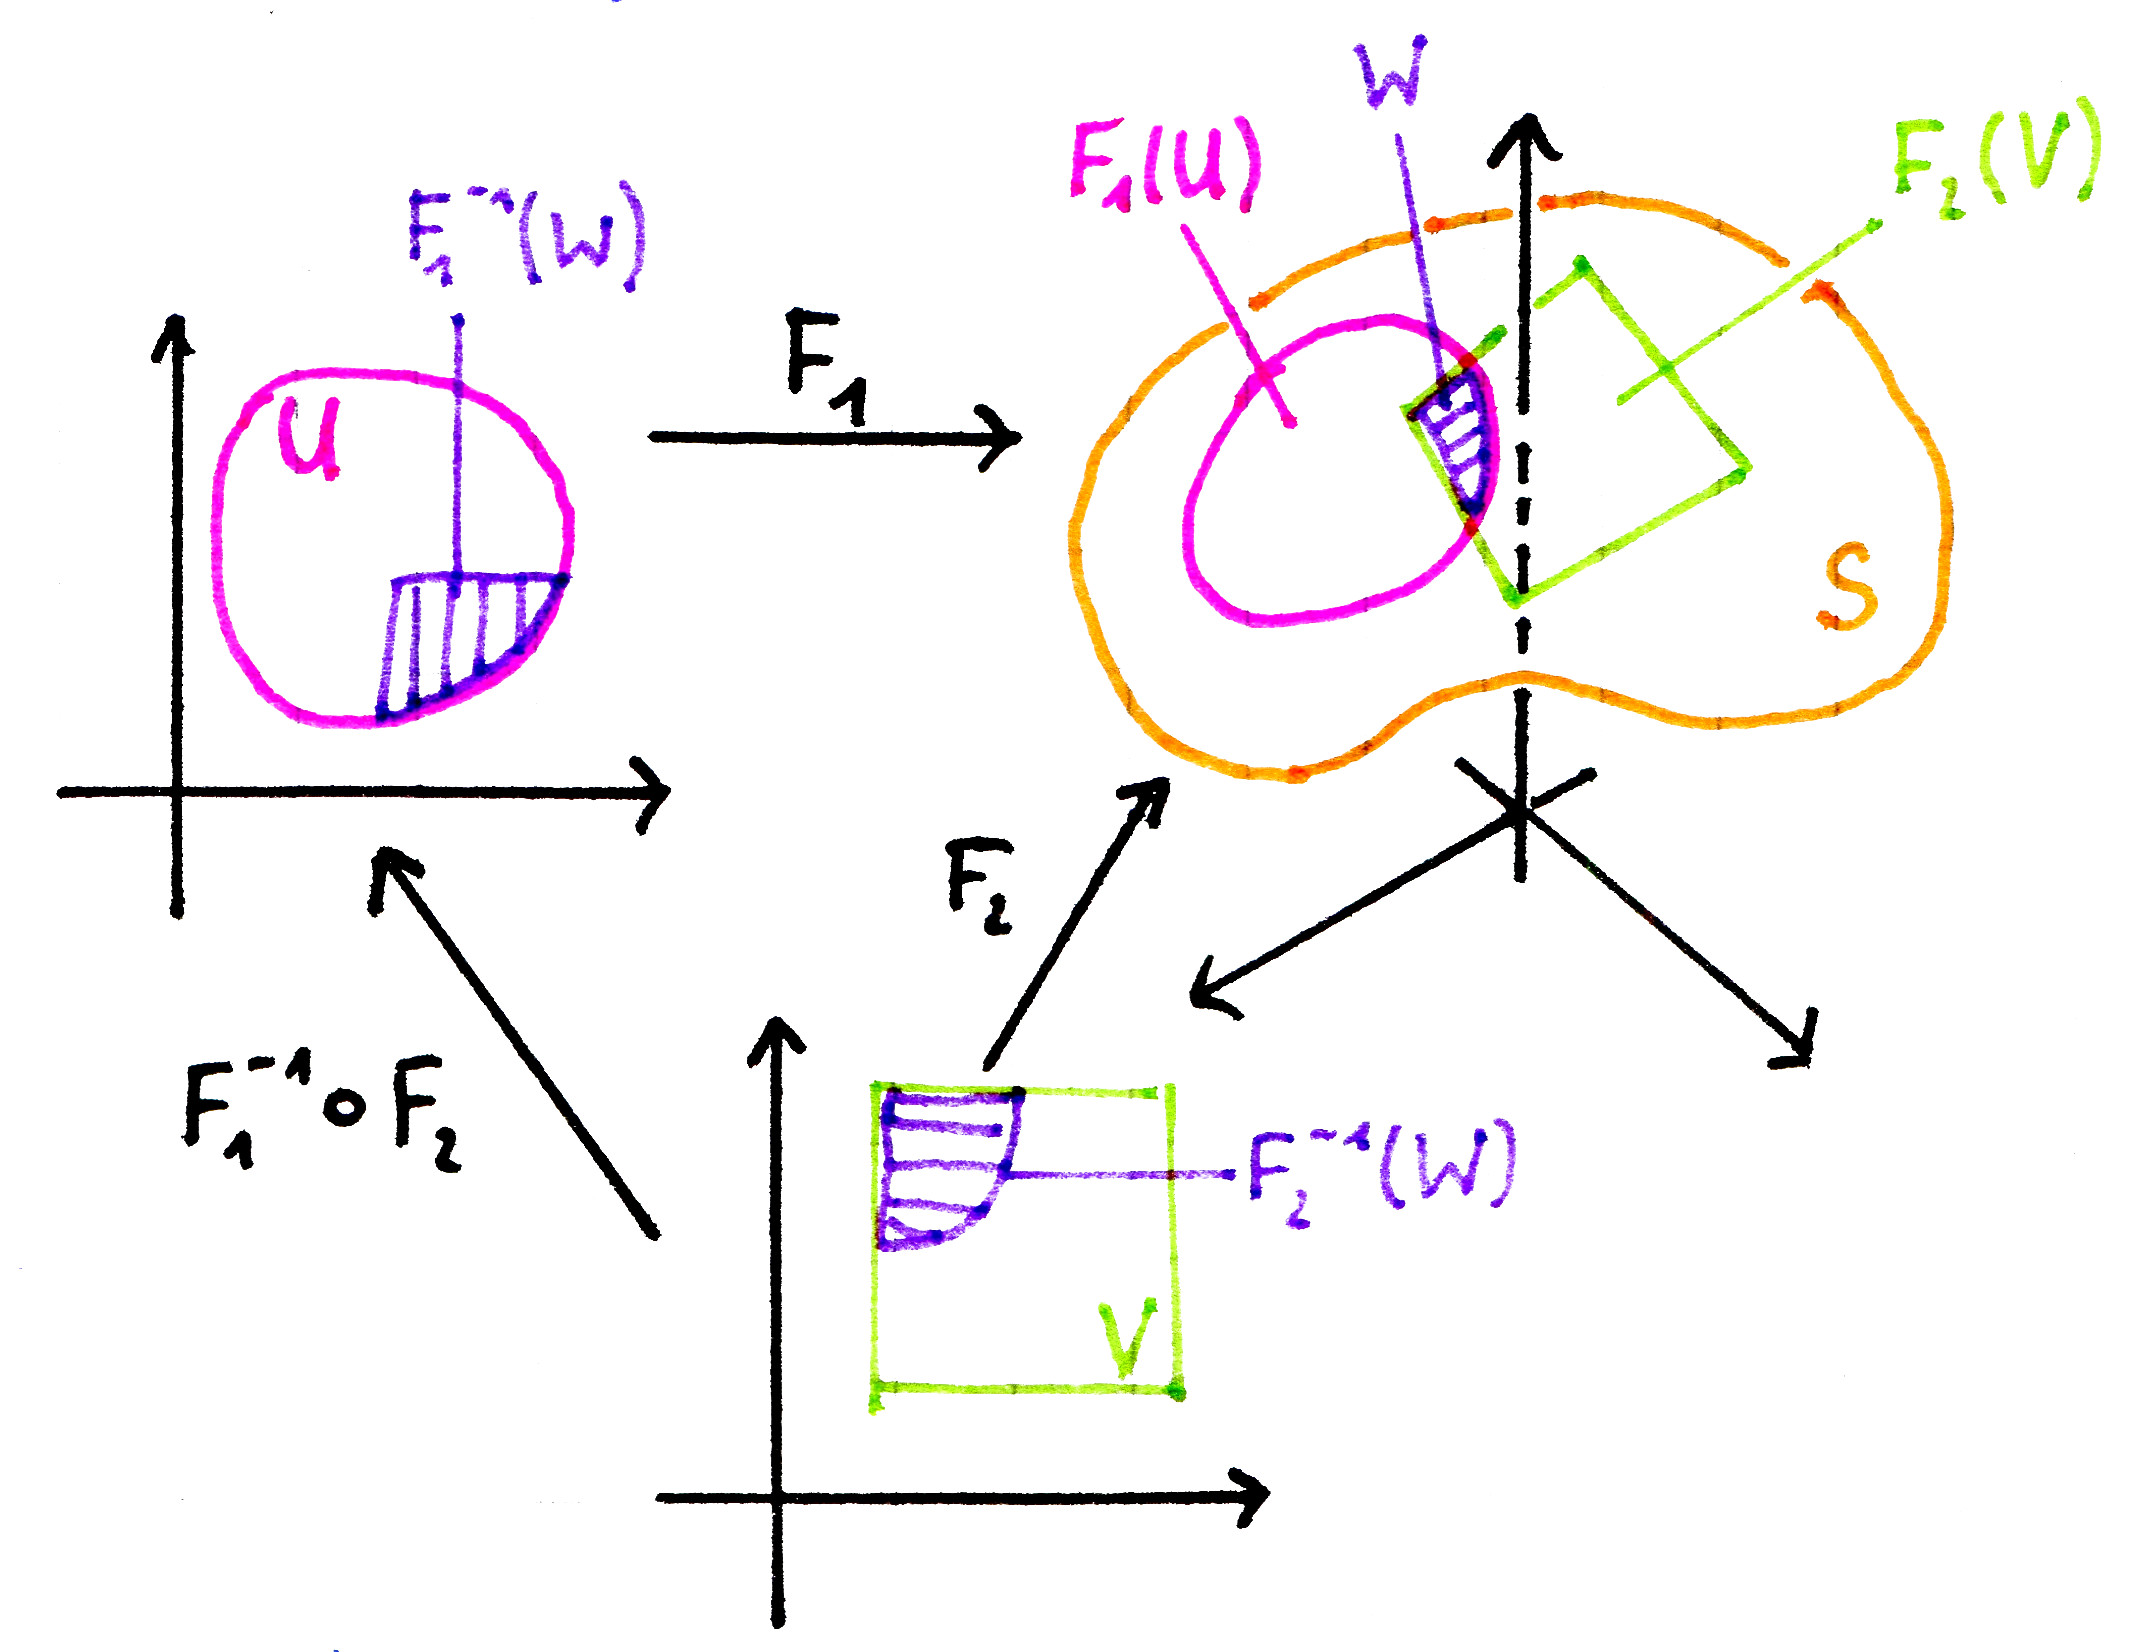
\includegraphics[width=.5\textwidth]{Parameterwechsel}
    \caption{Parameterwechsel}
  \end{figure}
  \begin{proof}
    \( H \) ist Homöomorphismus, da \( F_1 \) und \( F_2 \) Homöomorphismen sind. \\
    \emph{Problem}: \( F_1^{-1} \) ist auf einer offenen Teilmenge von \( S \) definiert und und da weiß man nicht was \emph{differenzierbar} heißt. \\
    \emph{Ausweg}: Erweiterung von \( F \). Sei \( r \in F_2^{-1}(W) \) und \( q \coloneqq H(r) \). Da
      \begin{equation*}
        F_1(u,v) = \left( x(u,v),y(u,v),z(u,v) \right)
      \end{equation*}
    reguläre Parametrisierung ist können wir oBdA (erst Koordinatenachsen von \( \R^3 \) umbenennen) annehmen, dass
    \begin{equation*}
      \frac{J(x,y)}{J(u,v)}(q) \neq 0 \quad \text{(Jacobi-Determinante).}
    \end{equation*}
    \emph{Trick}: Erweitere \( F_1 \) zu Abbildung
    \begin{align*}
      \widetilde{F_1} : U \times \R &\to \R^3 \\
        \widetilde{F_1}(u,v,t) &\coloneqq \left( x(u,v),y(u,v),z(u,v)+\bm{t} \right)\text{.}
    \end{align*}
    \( \widetilde{F_1} \) ist differenzierbar und \( \widetilde{F_1}|_{U \times \{ 0 \}} = F_1 \). \\
    Die Jacobi-Determinante von \( \widetilde{F_1} \) in \( (q,0) \),
    \begin{equation*}
      \det \begin{pmatrix}
        \frac{\text{d}x}{\text{d}u} & \frac{\text{d}x}{\text{d}v} & 0 \\
        \frac{\text{d}y}{\text{d}u} & \frac{\text{d}y}{\text{d}v} & 0 \\
        \frac{\text{d}z}{\text{d}u} & \frac{\text{d}z}{\text{d}v} & 1
      \end{pmatrix}(q,0) = \det \begin{pmatrix}
        \frac{\text{d}x}{\text{d}u} & \frac{\text{d}x}{\text{d}v} \\
        \frac{\text{d}y}{\text{d}u} & \frac{\text{d}y}{\text{d}v}
      \end{pmatrix}(q) \neq 0\text{.}
    \end{equation*}
    Nach dem Umkehrsatz (Analysis II) existiert eine Umgebung \( A \) von \( \widetilde{F_1}(q,0) = F_1(q) \) in \( \R^3 \) sodass \( \widetilde{F_1}^{-1} \) auf \( A \) existiert und differenzierbar (\( C^\infty \)) ist. Da \( F_2 \) stetig ist existiert Umgebung \( B \) von \( v \) in \( V \), sodass \( F_2(B) \subset A \). Und nun ist \( H|_B = \widetilde{F_1}^{-1} \circ F_2|_B \) ist Verkettung von differenzierbaren Abbildungen, also differenzierbar in \( r \) und da \( r \) beliebig ist ist \( H \) differenzierbar auf \( F_2^{-1}(W) \). \qed{}
  \end{proof}
\end{remark}

\begin{example}[Weitere Beispiele von differenzierbaren Mannigfaltigkeiten]
  \
  \begin{enumerate}
    \item \textbf{n-Sphäre} von Radius \( R \) (und Zentrum \( 0 \)):
      \begin{equation*}
        S_R^n \coloneqq \{ x \in \R^{n+1} : \Vert x \Vert = R \}\text{.}
      \end{equation*}
      Karten via stereographischer Projektion.
      \begin{align*}
        &N \coloneqq (0, \dots, 0, R), \quad &S \coloneqq (0, \dots, 0, -R) \\
        &U_1 \coloneqq S_R^n \setminus \{ N \}, \quad &U_2 \coloneqq S_R^n \setminus \{ S \}
      \end{align*}
      Stereographische Projektion bzgl \( N \):
      \begin{equation*}
        \phi_1 : U_1 \to \R^n, \ p = (p_1, \dots, p_{n+1}) \mapsto \left( x_1(p), \dots, x_n(p) \right), \ x_i(p) \coloneqq \frac{Rp_i}{R-p_{i+1}}
      \end{equation*}
      Stereographische Projektion bzgl. \( S \):\footnote{\textbf{Übung}: \( \phi_1 \) und \( \phi_2 \) sind Homöomorphismen.}
      \begin{equation*}
        \phi_1 : U_2 \to \R^n, \ p = (p_1, \dots, p_{n+1}) \mapsto \left( x_1(p), \dots, x_n(p) \right), \ x_i(p) \coloneqq \frac{Rp_i}{R-p_{i+1}}
      \end{equation*}
      Kartenwechsel:
      \begin{equation*}
        \phi_2 \circ \phi_1^{-1} : \R^n \setminus \{ 0 \} \to \R^n \setminus \{ 0 \}, \ \phi_2 \circ \phi_1^{-1}(x) = \frac{x}{\Vert x \Vert}R^2
      \end{equation*}
      ist \( C^\infty \). \\
      \( \Rightarrow \mathcal{A} \coloneqq \{ (U_1, \phi_1), (U_2, \phi_2) \} \) ist ein differenzierbarer Atlas für \( S_R^n \). \\
      \( \leadsto \) maximaler Atlas aller mit \( \mathcal{A} \) verträglichen Karten (also allen \( (U, \phi) \) mit \( \phi \circ \psi^{-1} \) ist \( C^\infty \) für \( \psi \) aus \( \mathcal{A} \) sofern Verkettung definiert ist) definiert differenzierbare Struktur auf \( S_R^n \), also ist \( S_R^n \) eine \( C^\infty \)-Mannigfaltigkeit mit Dimension \( n \).
    \item \( n \)-dimensionaler reell projektiver Raum
      \begin{equation*}
        P^n\R \coloneqq \{ \text{1-dim. UVR von } \R^{n+1} \} \equiv \left( \R^{n+1} \setminus \{ 0 \} \right) /\sim
      \end{equation*}
      mit \( x \sim y \overset{\text{Def.}}{\Leftrightarrow} \ \exists \ \R \ni \lambda \neq 0 : x = \lambda y \) (\( 1 \)-dimensionaler UVR = Äquivalenzklasse) \( \equiv S^n/\sim \) mit \( x \sim y \overset{\text{Def.}}{\Leftrightarrow} x = -y \). \\
      Wir sehen: \\
      \emph{1. Definition}: Eindimensionale Untervektorräume \\
      \emph{2. Definition}: Äquivalenzklassen in \( \R^{n+1} \setminus \{ 0 \} \) \\
      \emph{3. Definition}: Äquivalenzklassen in \( S^n \) \\
      Es ist leicht zu sehen, dass diese Definitionen äquivalent sind. \\
      Aus der 3. Definition sieht man
      \begin{equation*}
        P^n\R = S^n/\sim
      \end{equation*}
      ist kompakt als Quotientenraum von \( S^n \) (Quotiententopologie \( X \overset{\pi}{\to} Y = X/\sim \) mit topologischem Raum \( X \) und Quotiententopologie: \( U \) offen in \( Y \Leftrightarrow \pi^{-1}(U) \) ist offen in \( X \)). Diese Abbildung ist stetig, und ein stetiges Bild von einer kompakten Menge ist wieder kompakt. \\
      \textbf{Karten}:
      \begin{align*}
        \tilde{U_i} &\coloneqq \{ x \in S^n : x_i \neq 0 \}, \quad i = 1, \dots, n+1 \\
        U_i &\coloneqq \pi(\tilde{U_i}) \text{ mit } \pi: S^n \to S^n/\sim = P^n\R\text{.}
      \end{align*}
      Projektion:
      \begin{equation*}
        \phi_i : U_i \to \R^n, \quad \phi_i([x]) \coloneqq \left( \frac{x_i}{x_i}, \dots, \frac{x_{i-1}}{i}, \frac{x_{i+1}}{i}, \dots, \frac{x_n}{x_i} \right)
      \end{equation*}
      sind Homöomorphismen.\footnote{\textbf{Übung}: Kartenwechsel \( \phi_i \circ \phi_j^{-1} \) sind \( C^\infty \).}
  \end{enumerate}
\end{example}

\begin{remark}
  Man kann zeigen: \( P^n\R \) ist hausdorffsch und hat eine abzählbare Basis der Topologie. Also ist \( P^n\R \) eine \( n \)-dimensionale \( C^\infty \)-Mannigfaltigkeit. \\
  \emph{Analog}: \( P^n\C \coloneqq \{ \text{komplexe \( 1 \)-dim. UVR von } C^{n+1} \} \) ist kompakte \( 2n \)-dimensionale \( C^\infty \)-Mannigfaltigkeit.
  \begin{figure}[H]
    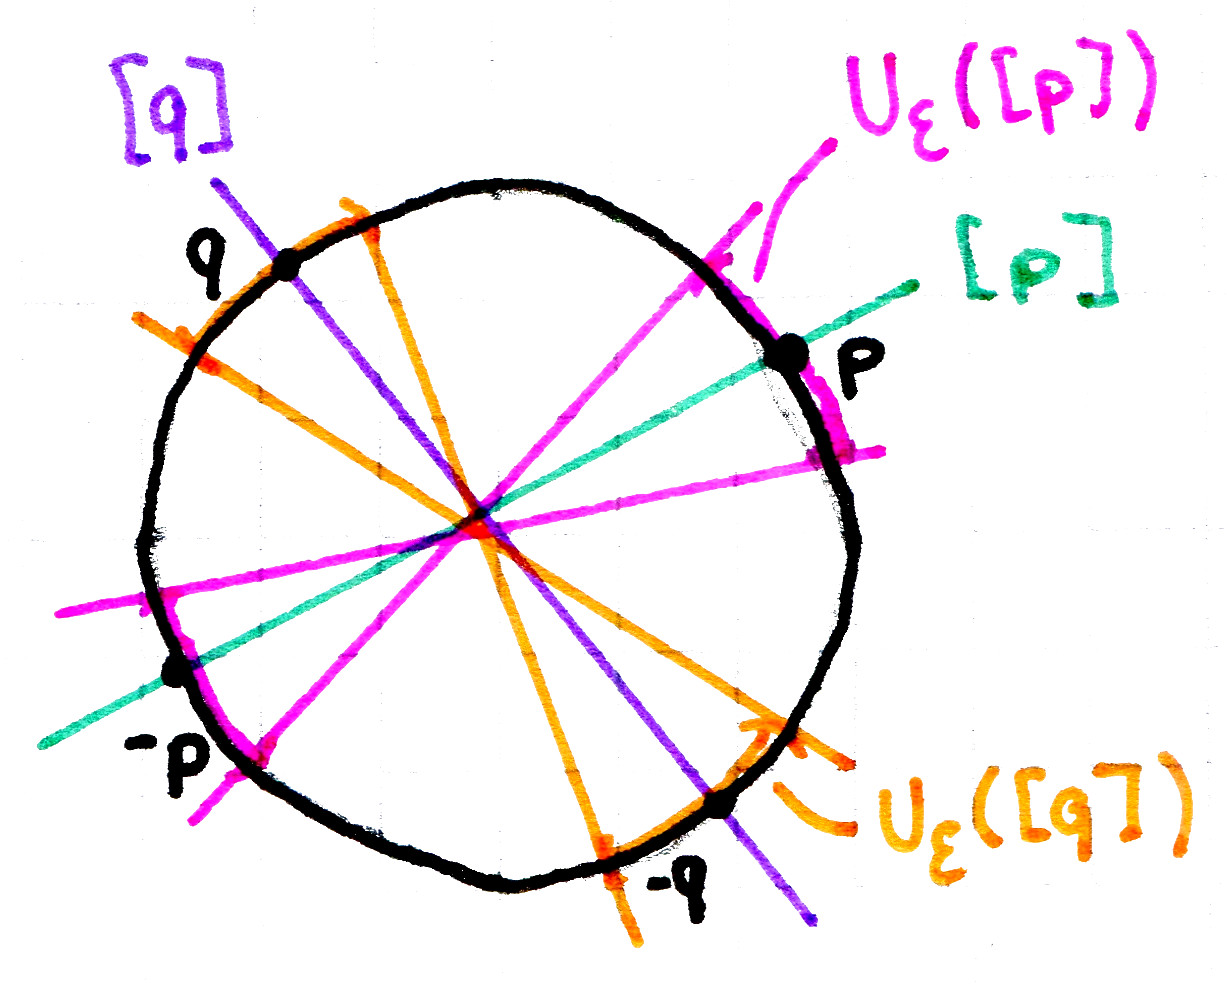
\includegraphics[width=.33\textwidth]{IdeeHausdorffsch}
    \caption{Idee zu Hausdorffsch}
  \end{figure}
\end{remark}

\begin{example}[Produkt-Mannigfaltigkeiten]
  Für \( M^m \) und \( N^n \) \( m \)- bzw. \( n \)-dimensionale differenzierbare Mannigfaltigkeit ist die \term{Produkt-Mannigfaltigkeit}\label{def:produktmannigfaltigkeit} \( M \times N \) eine \( (m+n) \)-dimensionale \( C^\infty \)-Mannigfaltigkeit.\footnote{\textbf{Übung}!}
\end{example}

\begin{excourse}[Lie-Gruppen]
  Eine \term{Lie-Gruppe}\label{def:liegruppe} ist eine Gruppe mit einer \( C^\infty \)-Mannigfaltigkeitstruktur, so dass die Abbildung
  \begin{equation*}
    G \times G \to G, \quad (g,h) \mapsto gh^{-1}
  \end{equation*}
  \( C^\infty \) ist.
\end{excourse}

\begin{example}[zu Lie-Gruppen]
  \
  \begin{itemize}
    \item \( (\Z, +) \) ist eine \( 0 \)-dimensionale Lie-Gruppe.
    \item \( SO(2) = \left \{ \begin{pmatrix}
      \cos \theta & -\sin \theta \\
      \sin \theta & \cos \theta
    \end{pmatrix} : \theta \in [0, 2\pi] \right \} \underset{\text{homö}}{\cong} S^1 \) ist kompakte \( 1 \)-dimensionale \( C^\infty \)-Mannigfaltigkeit und Lie-Gruppe.\footnote{\textbf{Übung}: Wieso?} 
    \item \( SU(2) \coloneqq \left \{ \begin{pmatrix}
      \alpha & \beta \\
      -\overline{\beta} & \overline{\alpha}
    \end{pmatrix} : \alpha, \beta \in \C, \ \alpha\overline{\alpha}+\beta\overline{\beta} = 1 \right \} \underset{\text{homö}}{\cong} S^3 \) ist kompakte \( 3 \)-dimensionale \( C^\infty \)-Mannigfaltigkeit.\footnote{\( 1 = \alpha\overline{\alpha}+\beta\overline{\beta} = x_1^2 + x_2^2 + x_3^2 + x_4^2 \) mit \( \alpha = x_1+\i x_2 \) und \( \beta = x_3 + \i x_4 \).}
    \item \( GL(n, \R) \) (offene) Untermannigfaltigkeit von \( \R^{n^2} \leadsto n^2 \)-dimensionale \( C^\infty \)-Mannigfaltigkeit.
  \end{itemize}
\end{example}

\begin{remark}[Fakt von Cartan]
  Abgeschlossene Untergruppen von Lie-Gruppen sind Lie-Gruppen sind auch Lie-Gruppen.
\end{remark}

\begin{example}[Fakt von Cartan benutzen]
  \
  \begin{align*}
    SO(n) &= \{ A \in GL(n, \R) : AA^\top = E, \ \det A = 1 \} \text{ und} \\
    SL(n, \R) &= \{ A \in GL(n, \R) : \det A = 1 \}
  \end{align*}
  sind Lie-Gruppen: Benutze, dass
  \begin{equation*}
    A = \{ x \in X : f(x) = g(x) \} \text{ und } X \text{ ist hausdorffsch}
  \end{equation*}
  \( \Rightarrow A \text{ abgeschlossen, } f, g \text{ stetige Abbildungen} \)
\end{example}

\section{Simplizialkomplexe}

Simplizialkomplexe sind Objekte der algebraischen Topologie. Mittels Kombinatorik sollen topologische Invarianten bestimmt werden.

\begin{definition}[Simplex]
  Ein \( k \)-dimensionales \term{Simplex}\label{def:simplex} im \( \R^n \) ist die konvexe Hülle von \( k+1 \) Punkten \( v_0, \dots, v_k \) in allgemeiner Lage:
  \begin{equation*}
    s(v_0, \dots, v_k) \coloneqq \left \{ \sum_{i=0}^n \lambda_i v_i : \forall \lambda_i \geq 0, \ \sum_{i = 0}^k \lambda_i = 1 \right \}
  \end{equation*}
  für \( v_0-v_1, \dots, v_0-v_k \) linear unabhängig.
\end{definition}

\begin{example}[Einfache Simplices]
  \
  \begin{itemize}
    \item \textbf{0-Simplex}: \( v_0 \) (Punkt) 
    \item \textbf{1-Simplex}: \( v_0 \) --- \( v_1 \) (Strecke, \( s(v_0, v_1) = \{ \lambda v_0 + (1-\lambda)v_1 : 0 \leq \lambda \leq 1 \} \))
    \item \textbf{2-Simplex}: \( \triangle v_0, v_1, v_2 \) (Dreiecksfläche)
    \item \textbf{3-Simplex}: \( v_0, v_1, v_2, v_3 \) ((volles) Tetraeder)
  \end{itemize}
  \begin{figure}[H]
    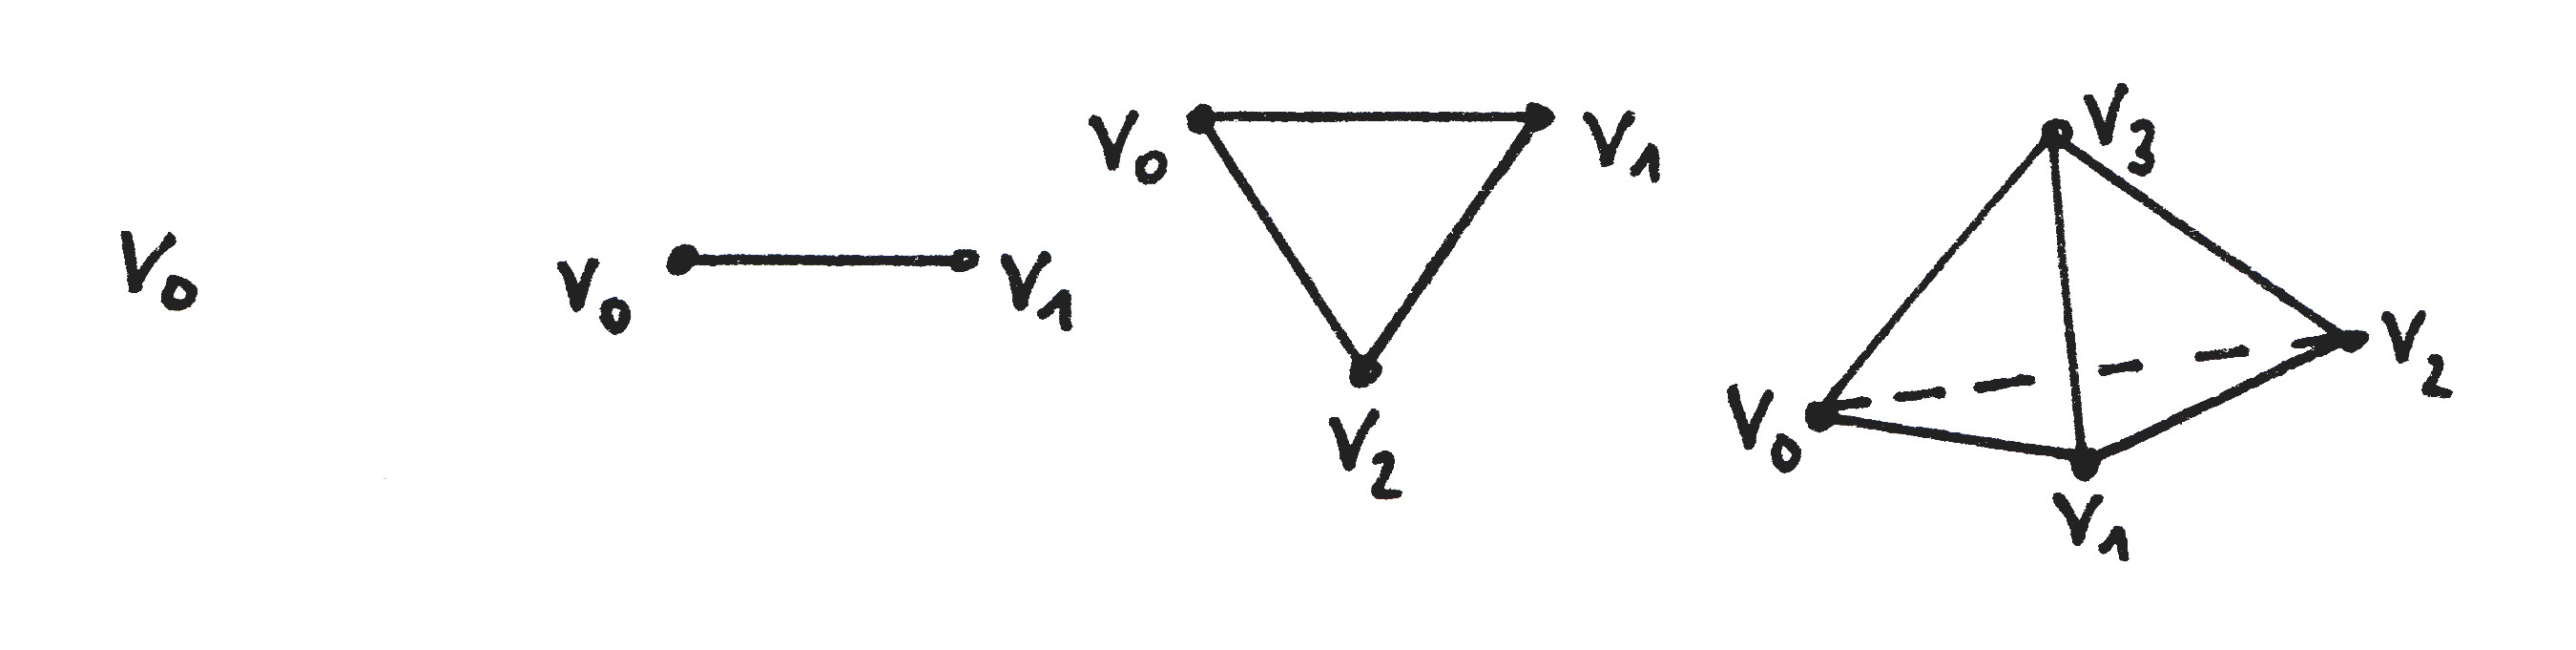
\includegraphics[width=.5\textwidth]{0123Simplex}
    \caption{\( 0 \)-, \( 1 \)-, \( 2 \)- und \( 3 \)-Simplex}
  \end{figure}
\end{example}

\begin{minipage}{.45\textwidth}
  \begin{definition}[Teilsimplex, Seite]
    Die konvexe Hülle einer Teilmenge von \( \{ v_0, \dots, v_k \} \) heißt \term{Teilsimplex}\label{def:seite} oder \term{Seite} von \( s(v_0, \dots, v_k) \).
  \end{definition}
\end{minipage}
\hfill
\begin{minipage}{.45\textwidth}
  \begin{figure}[H]
    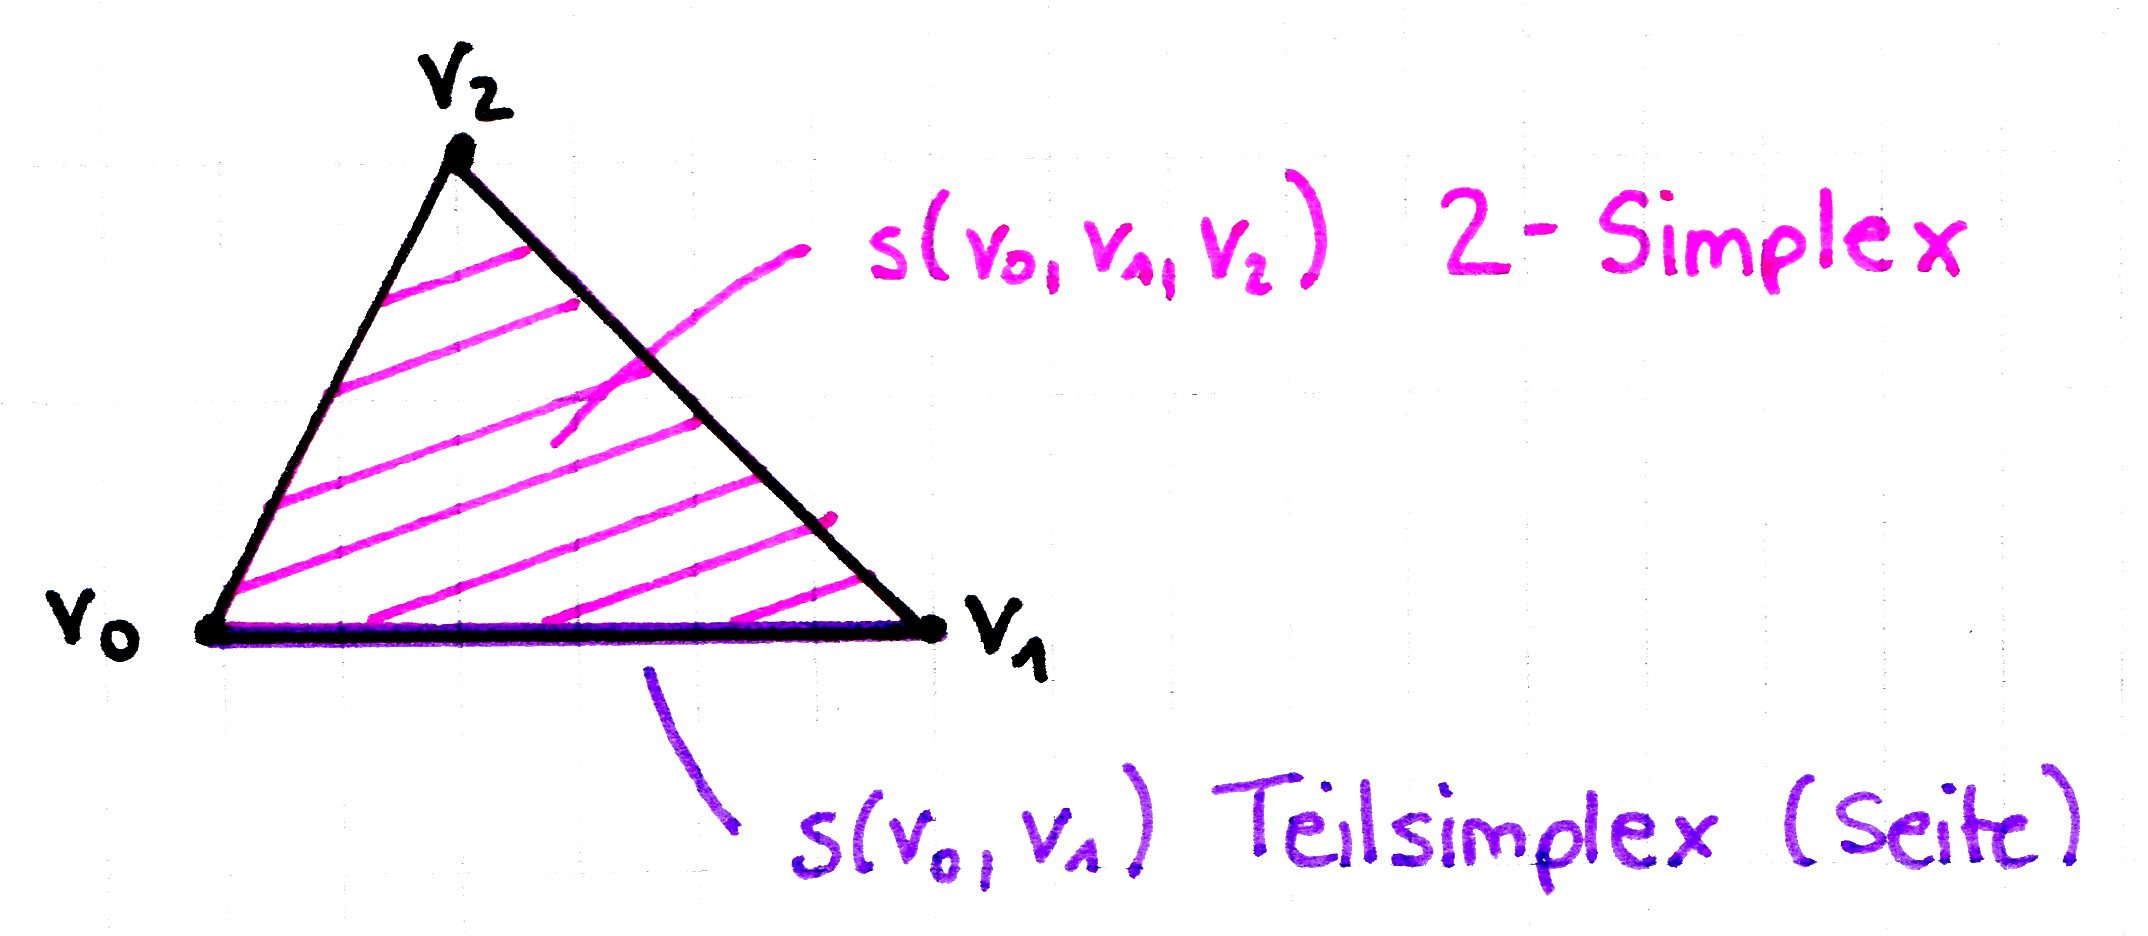
\includegraphics[width=\textwidth]{SimplexTeilsimplex}
    \caption{Simplex und Teilsimplex}
  \end{figure}
\end{minipage}

\begin{definition}[Simplizialkomplex]
  Eine endliche Menge \( K \) von Simplices in \( \R^n \) heißt \term{Simplizialkomplex}\label{def:simplizialkomplex}, wenn gilt:
  \begin{enumerate}
    \item Mit jedem seiner Simplices enthält \( K \) auch dessen sämtliche Teil-Simplices.
    \item Der Durchschnitt von je zwei Simplices ist entweder leer oder ein gemeinsamer Teilsimplex. 
  \end{enumerate}
  \begin{figure}[H]
    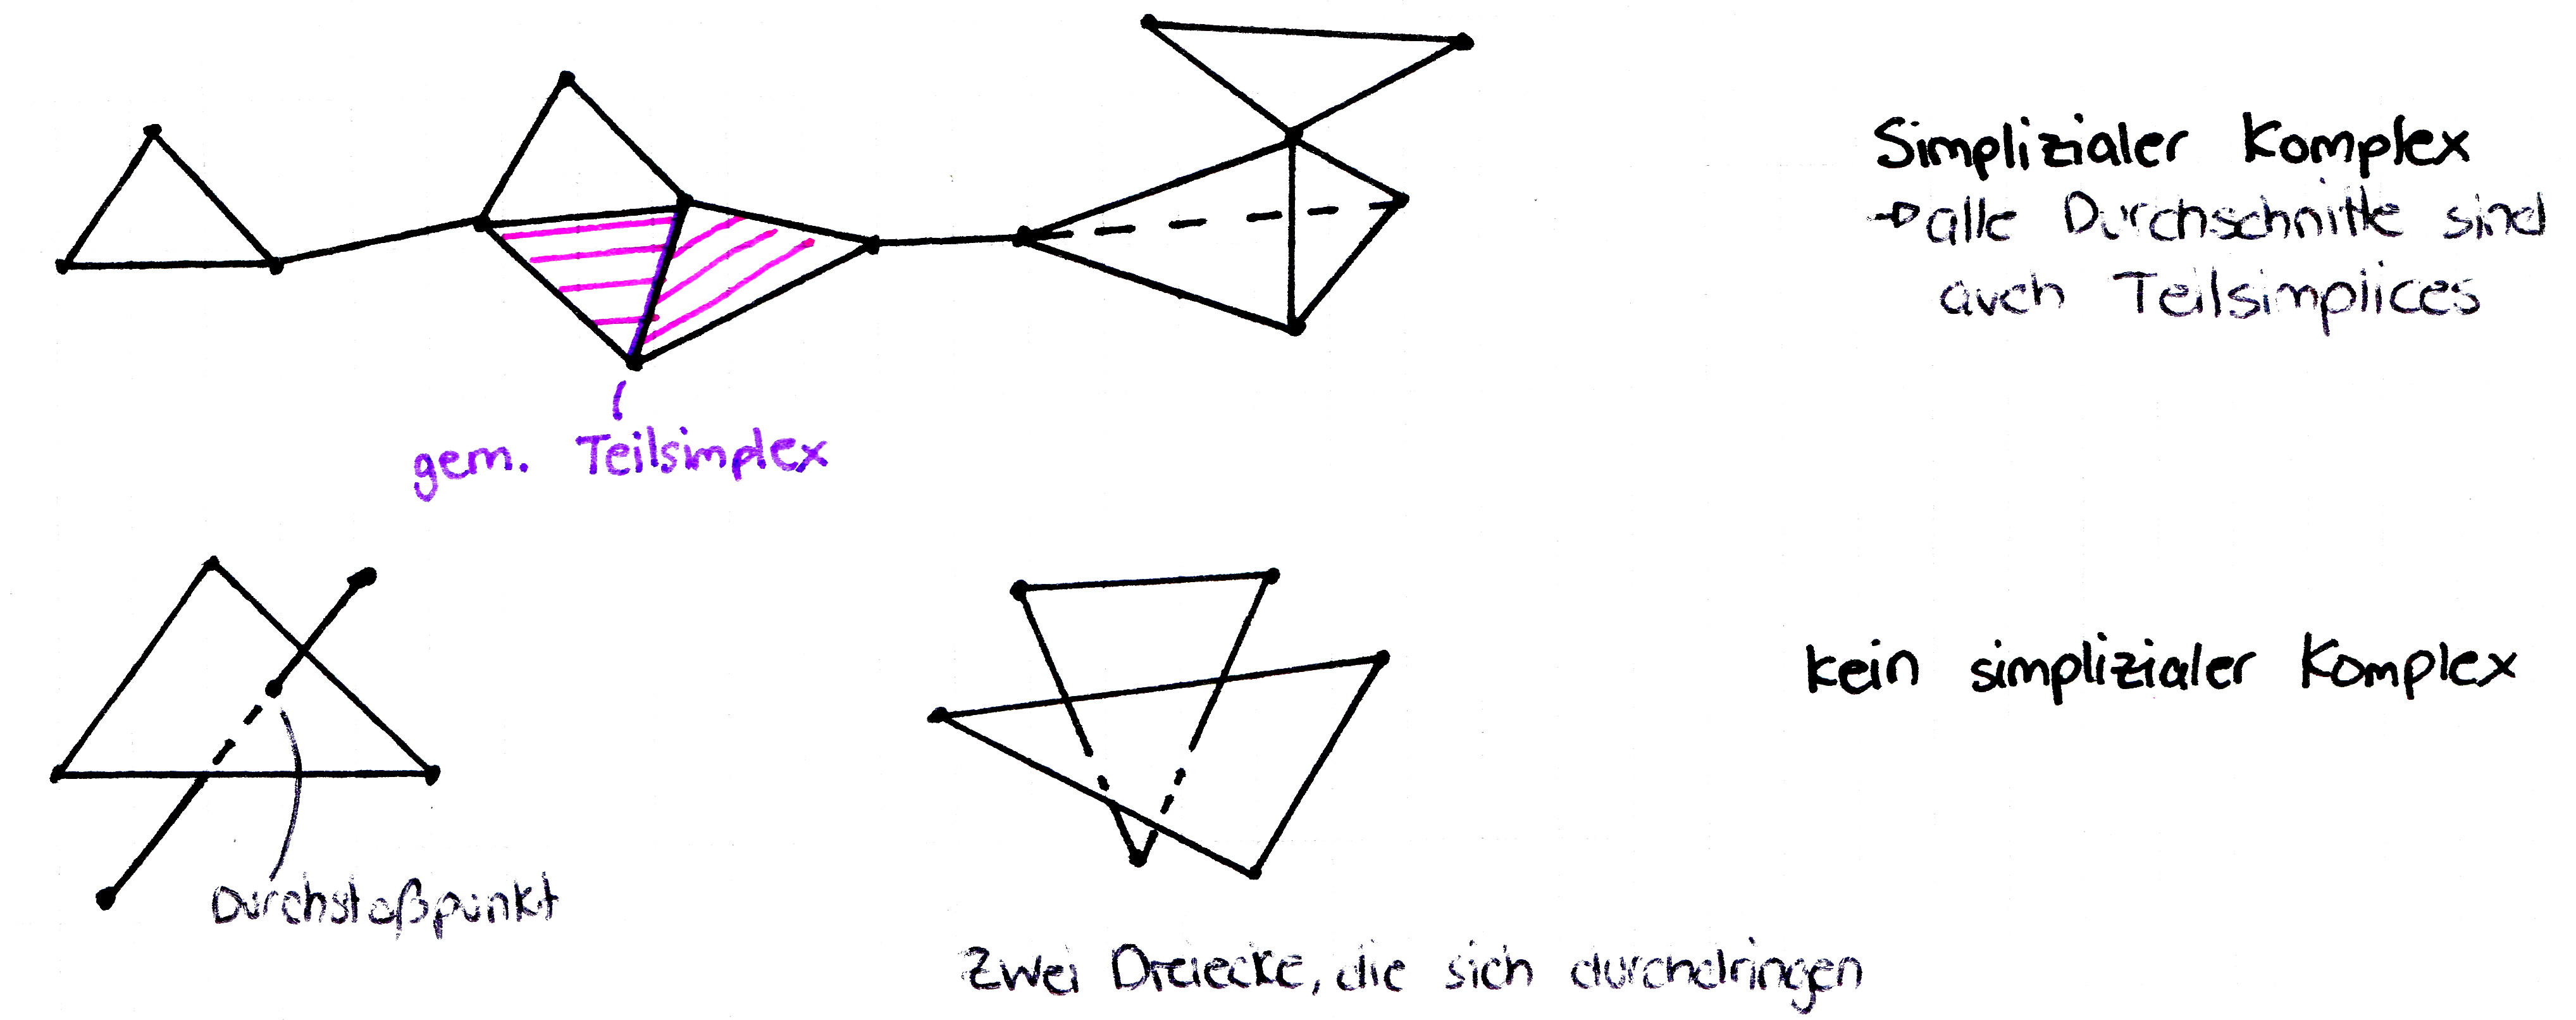
\includegraphics[width=.8\textwidth]{KeinSimplizialkomplex}
    \caption{Simplizialkomplex versus kein Simplizialkomplex}
  \end{figure}
\end{definition}

\begin{definition}[Geometrische Realisierung]
  \
  \begin{equation*}
    \vert K \vert \coloneqq \bigcup_{s \in K} s \subset \R^n
  \end{equation*}
  mit Teilraumtopologie von \( \R^n \) heißt der dem Simplizialkomplex \( K \) zugrunde liegende topologische Raum. \\
  \emph{Achtung}: Verschiedene Simplizialkomplexe \( K \), \( K' \) können das gleiche \( \vert K \vert = \vert K' \vert \) haben.
  % TODO Abbildung 1
\end{definition}

\begin{remark}[Vorteil von Simplizialkomplexen]
  Kennt man von einem (endlichen) Simplizialkomplex die \term{wesentlichen Simplices}\label{def:wesentlicheSimplices} (also solche, die nicht Seiten von anderen sind) in jeder Dimension und ihre \term{Inzidenzen}\label{def:inzidenzen} (also welche Ecken sie gemeinsam haben), so kennt man \( \vert K \vert \) (bis auf Homöomorphie).
  \begin{proof}[Konstruktionsidee von \( \vert K \vert \) aus diesen Daten]
    \
    \begin{enumerate}
      \item Wähle in jeder Dimension einen \emph{Standard-Simplex} \( \Delta_k \coloneqq s(\underbrace{e_1, \dots, e_{k+1}}_{\text{Std.-Basis-Vek.}}) \)
      \item Bilde disjunkte Vereinigung von solchen \( \Delta_k \) in jeder Dimension \( k \) so viele wie es wesentliche \( k \)-Simplices gibt:
        \begin{equation*}
          X \coloneqq \underbrace{\Delta_0 \cup \dots \cup \Delta_0}_{\text{\# wesentliche \( 0 \)-Simp.}} \cup \dots \cup \underbrace{\Delta_n \cup \dots \cup \Delta_n}_{\text{\# wesentliche \( n \)-Simp.}}
        \end{equation*}
      \item Identifiziere Inzidenzen (via Äquivalenzrelation) gemäß Inzidenz-Angaben für Ecken
    \end{enumerate}
    Diese drei Schritte liefern dann eine stetige Bijektion des (kompakten) Quotientenraumes \( X/\sim \) auf Hausdorff-Raum \( \vert K \vert \), also ein Homöomorphismus. \qed{}
  \end{proof}
\end{remark}

\begin{definition}[Dimension]
  Die \term{Dimension} eines Simplizialkomplexes \( K \) ist die maximale Dimension seiner Simplices.
\end{definition}

\begin{remark}[Spezialfall --- Graph]
  Ein \term{endlicher Graph}\label{def:graph} ist ein endlicher, \( 0 \)- oder \( 1 \)-dimensionaler Simplizialkomplex,\footnote{Aufgrund der Eindimensionalität haben beispielsweise die Dreiecke in einem Graph keine Füllung!} gebaut aus \( 1 \)-dimensionalen (\emph{Kanten}) und \( 0 \)-dimensionalen (\emph{Ecken}) Simplices. \\
  Ein Graph \( G \) heißt \term{zusammenhängend}\label{def:zusammenhaengend}, falls zu je zwei Ecken \( p, p' \in G \) eine Folge \( p = p_0, p_1, \dots, p_n = p' \) paarweise verschiedener Ecken von \( G \) existiert, sodass \( p_{i-1} \) und \( p_i \) durch eine Kante verbunden sind. \\
  Ein \term{Baum}\label{def:baum} ist ein zusammenhängender Graph \( T \), so dass für jedes \( 1 \)-Simplex (\emph{Kante}) \( s \in T \) gilt: \( \vert T \vert \setminus \mathring{s} \) ist nicht zusammenhängend (mit \( \mathring{s} = \) \emph{offener} \( 1 \)-Simplex, also Kante ohne Endpunkte).
\end{remark}

\begin{definition}[Euler-Charakteristik]
  Sei \( G \) ein endlicher Graph,
  \begin{align*}
    \alpha_0 &\coloneqq \text{ Anzahl Ecken in } G\text{,} \\
    \alpha_1 &\coloneqq \text{ Anzahl Kanten in } \text{G.}
  \end{align*}
  Die \term{Euler-Charakteristik}\label{def:eulerCharakteristik} von \( G \) ist
  \begin{equation*}
    \chi(G) \coloneqq \alpha_0 - \alpha_1
  \end{equation*}
  \emph{Bemerkung}: \( \chi(G) \) ist invariant unter Unterteilung (also dem Hinzufügen von neuen Ecken auf einer Kante).
\end{definition}

\begin{theorem}[\( \chi \) von Bäumen]
  Sei \( T \) ein (endlicher) Baum. Dann gilt \( \chi(T) = 1 \).
  \begin{proof}
    Induktion nach \( \alpha_0 = \) Anzahl Ecken.
    \begin{itemize}
      \item \( n = 1 \). Dann ist \( G \) ein Punkt, \( \alpha_0 = 1 \), \( \alpha_1 = 0 \), \( \chi(T) = \alpha_0 - \alpha_1 = 1 \quad \checkmark \)
      \item \( n = 2 \). Dann ist \( G \) eine Kante mit Endpunkten, \( \alpha_0 = 2 \), \( \alpha_1 = 1 \), \( \chi(T) = 1 \quad \checkmark \)
      \item \textbf{Induktionsannahme}: Satz gilt für alle Bäume mit \( n \) Ecken.
      \item \textbf{Induktionsschritt}: \( \chi(T) = 1 \) für Bäume mit \( n+1 \) Ecken. \\
        Sei \( T \) ein Baum mit \( n+1 \) Ecken und \( v_0 \) ein \term{Ende}\label{def:blatt} von \( T \) (also eine Ecke die zu genau einer Kante gehört). Ein solches Ende existiert.\footnote{vgl. Übung} \\
        Sei \( \vert T_1 \vert \coloneqq \vert T \vert \setminus \{ \mathring{s_1} \cup v_0 \} \). \( T_1 \) ist wieder ein Baum, sonst existiert \( s_2 \) sodass \( T_1 \setminus \{ \mathring{s_2} \} \) zusammenhängend ist, also auch \( T \setminus \{ \mathring{s_2} \} \) zusammenhängend \( \lightning \). \\
        \( T_1 \) hat \( n \) Ecken, also nach IV:\@ \( \chi(T_1) = 1 \). \\
        Da \( \alpha_0(T) = \alpha_0(T_1) + 1 \) und \( \alpha_1(T) = \alpha_1(T_1) + 1 \) ist \( \chi(T_1) = 1 \). \qed{}
    \end{itemize}
  \end{proof}
\end{theorem}

\begin{theorem}[\( \chi \) von zusammenhängenden Graphen]
  Sei \( G \) ein zusammenhängender, endlicher Graph. Sei \( n \) die Anzahl von offenen \( 1 \)-Simplices (\emph{Kanten}), die man aus \( G \) entfernen kann, sodass \( G \) zusammenhängend bleibt. Dann ist \( \chi(G) = 1 - n \).\footnote{Die Aussage aus dem vorhergehenden Satz folgt aus diesem direkt.}
  \begin{proof}
    Ist \( G \) ein Baum, so ist \( n = 0 \) und die Behauptung gilt. \\
    Ist \( G \) \underline{kein} Baum, so existiert ein offenes \( 1 \)-Simplex \( \mathring{s_1} \), sodass \( \vert G_1 \vert = \vert G \vert \setminus \{ \mathring{s_1} \} \) zusammenhängend ist. Ist \( G_1 \) ein Baum, so hält man an. Ist \( G_1 \) kein Baum, so entfernt man eine Kante \( \mathring{s_2} \) und so weiter. \\
    \( G \) hat endlich viele Kanten, also existiert ein maximales \( n \), so dass \( \vert G \vert \setminus \{ \mathring{s_1} \cup \cdots \cup \mathring{s_n} \} \) ein Baum ist. \\
    Es gilt dann \( \chi(G) = \chi(T) - n = 1-n \). \qed{}
  \end{proof}
  \emph{Bemerkung}: Das Komplement \( T \) aller offenen Kanten die man aus \( G \) entfernen kann (wie im Beweis) ist ein sog. \term{spannender Baum}\label{def:spannenderBaum} für \( G \), der alle Ecken in \( G \) enthält (nicht eindeutig).
\end{theorem}

\begin{definition}[Ebene und planare Graphen]
  Ein Graph heißt \term{eben}\label{def:eben}, falls er durch Punkte und Geradenstücke in der Ebene (also \( \R^2 \)) realisiert ist, so dass sich die Kanten nicht schneiden (außer in den Ecken). \\
  Ein (abstrakter) Graph (also gegeben durch Ecken-Mengen und Inzidenzen) heißt \term{planar}\label{def:planar}, falls er \emph{isomorph} zu einem ebenen Graphen ist.  
\end{definition}

\begin{example}
  \
  \begin{enumerate}
    \item \( K_4 = \) vollständiger Graph mit \( 4 \) Ecken (also sind alle Ecken-Paare durch Kanten verbunden). Zeichnet man diesen Graphen als Quadrat, so ist dieser nicht eben. Man kann aber \( K_4 \) so zeichnen, dass der Graph eben ist. Also ist \( K_4 \) planar.
    \item \( K_5 = \) vollständiger Graph mit \( 5 \) Ecken. Dieser Graph ist nicht isomorph zu einem ebenen Graphen, also ist \( K_5 \) nicht planar.
  \end{enumerate}
  \begin{figure}[H]
    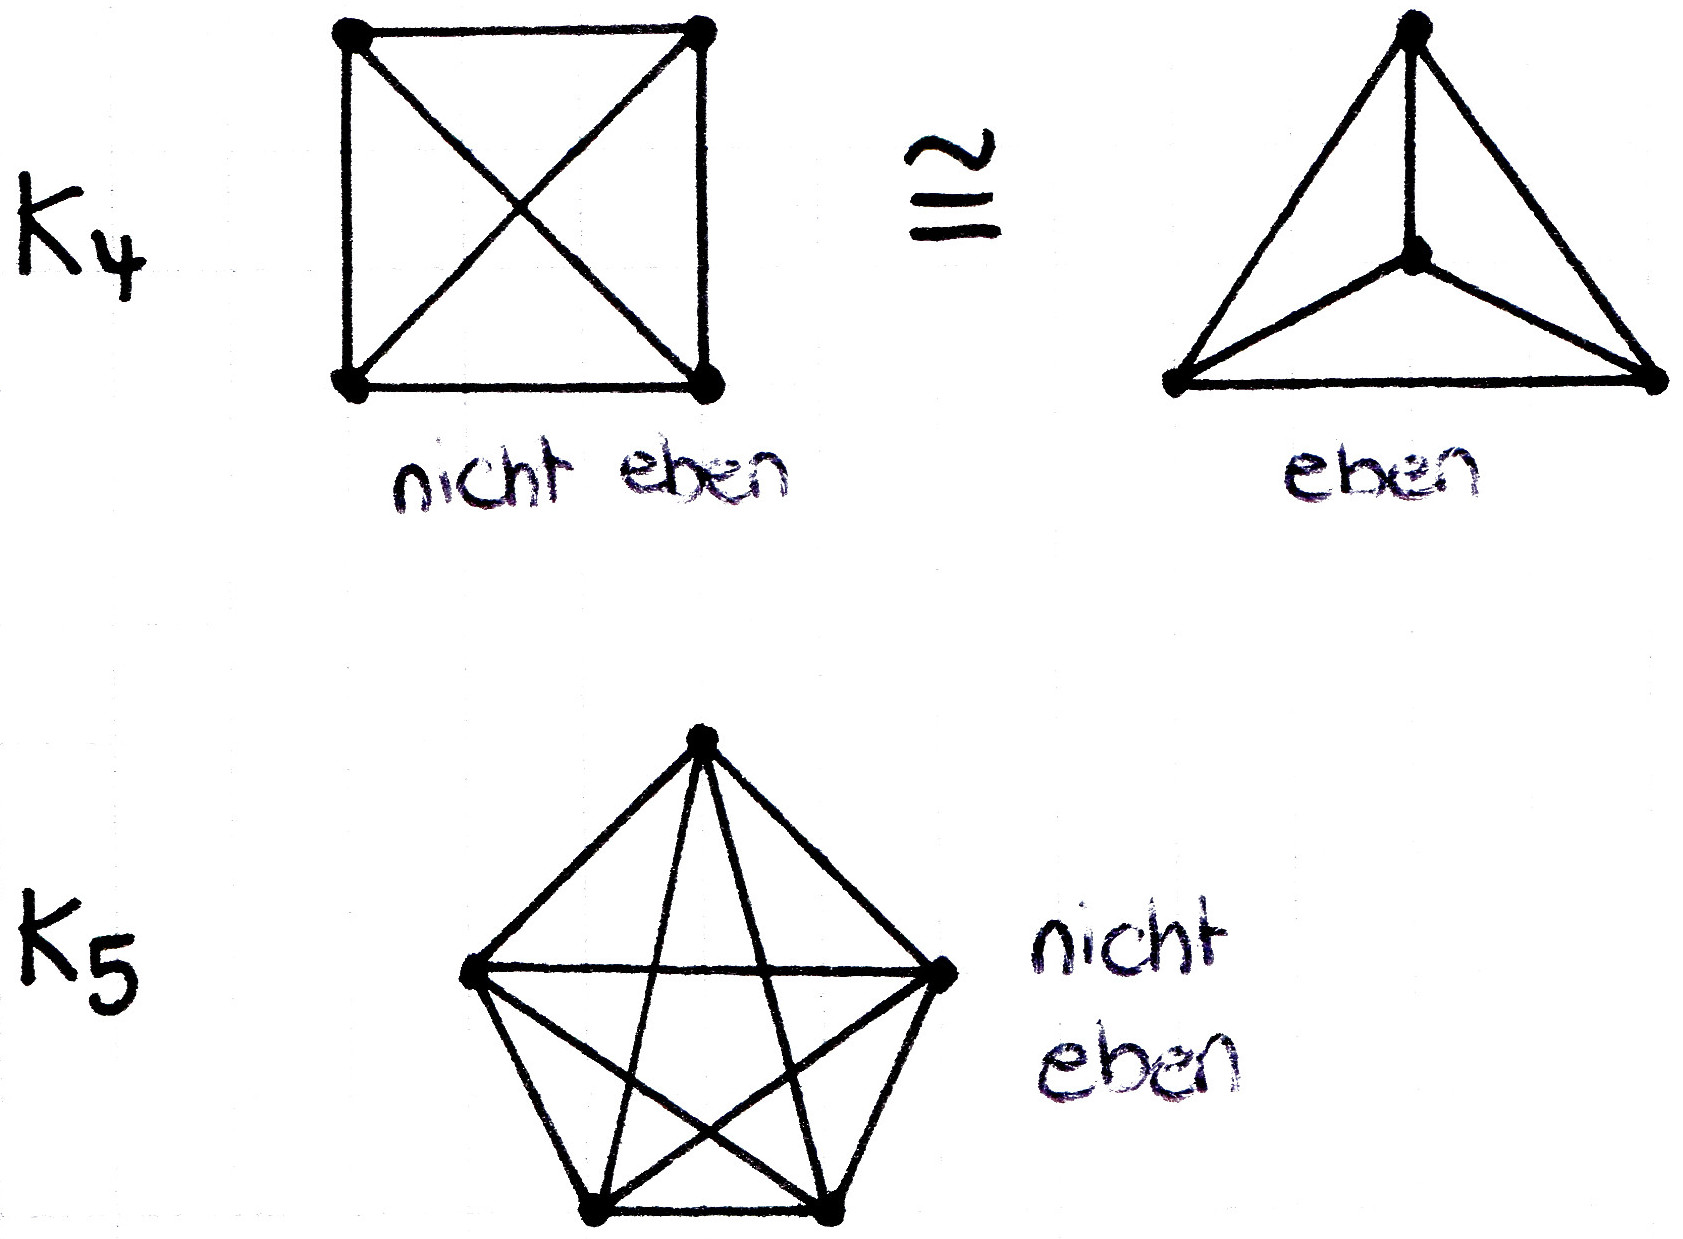
\includegraphics[width=.33\textwidth]{NichtPlanar}
    \caption{Planar versus nicht planar}
  \end{figure}
\end{example}

\begin{minipage}{.45\textwidth}
  \begin{definition}[Seiten]
    Die \term{Seiten}\label{def:seiten} eines ebenen Graphen \( G \) sind die Zusammenhangskomponenten von \( \R^2 \setminus G \).
  \end{definition}
\end{minipage}
\hfill
\begin{minipage}{.45\textwidth}
  \begin{figure}[H]
    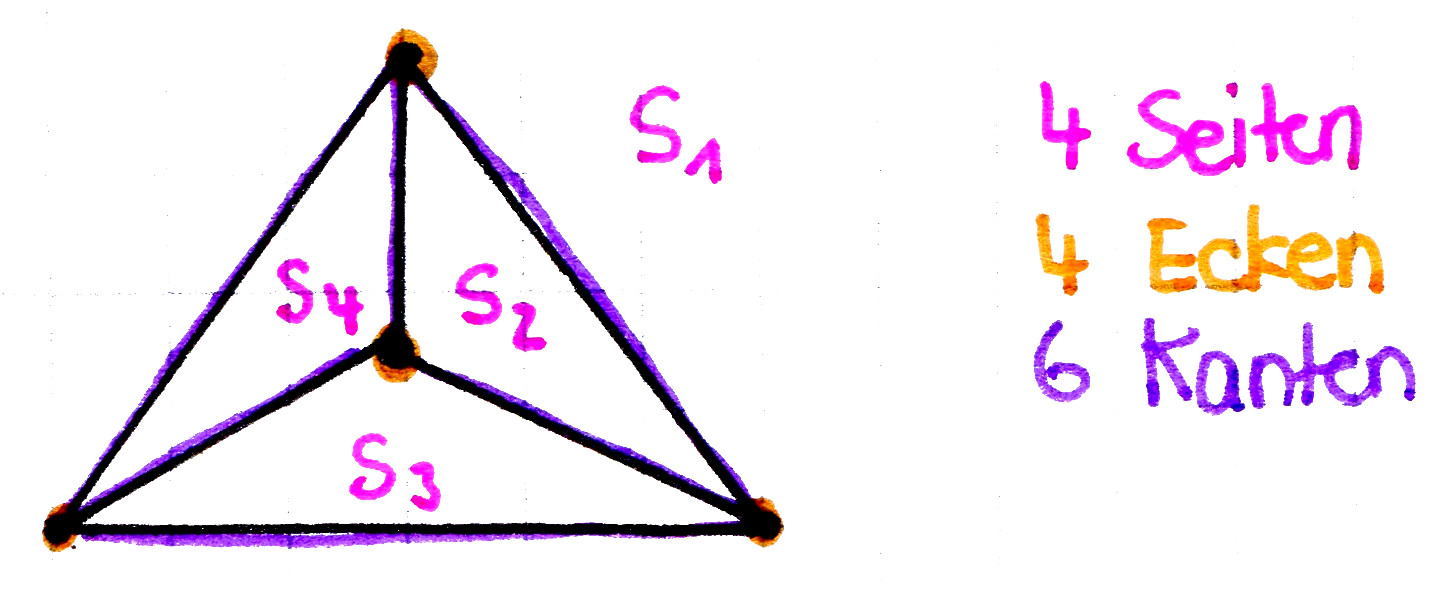
\includegraphics[width=.8\textwidth]{SeitenEckenKanten}
    \caption{Seiten, Ecken und Kanten eines Graphen}
  \end{figure}
\end{minipage}

\begin{theorem}[Euler-Formel]
  Für einen zusammenhängenden, ebenen Graphen \( G \) gilt:
  \begin{equation*}
    \chi(G) \coloneqq e(G) - k(G) + s(G) = 2\text{,}
  \end{equation*}
  wobei \( e(G) \) die Anzahl Ecken von \( G \), \( k(G) \) die Anzahl Kanten von \( G \) und \( s(G) \) die Anzahl Seiten von \( G \) ist. \\
  \( \chi(G) \) ist die \term{Euler-Charakteristik}\label{def:eulercharakteristik} von \( G \).
  \begin{proof}
    Sei \( T \) ein \term{aufspannender Baum}\label{def:aufspannenderBaum} für \( G \) (also ein Baum der alle Ecken von \( G \) enthält). Dann gilt \( e(T)-k(T) = 1 \) und \( s(T) = 1 \). Also gilt die Behauptung für \( T \). \\
    \( G \) erhält man aus \( T \) durch Hinzufügen von Kanten. Für jede neue Kante entsteht auch eine neue Seite, welche sich in der Summe aus der Behauptung aufheben. Also
    \begin{equation*}
      \chi(G) = e(G)-k(G)+s(G) = 2\text{.}
    \end{equation*}\qed{}
  \end{proof}
\end{theorem}

\begin{definition}[Polyeder]
  Eine Teilmenge \( P \) von \( \R^3 \) heißt \term{(konvexes) Polyeder}\label{def:polyeder}, falls
  \begin{enumerate}
    \item \( P \) ist Durchschnitt von endlich vielen \term{affinen Halbräumen}\label{def:affinerHalbraum} von \( \R^3 \) (also gegeben durch Ungleichungen \( {a_i}x+{b_i}y+{c_i}z \geq d_i \), \( i = 1, \dots, k \))
    \item \( P \) ist beschränkt und nicht in einer Ebene enthalten.
  \end{enumerate}

  \begin{minipage}{.45\textwidth}
    Der \term{Rand}\label{def:rand} von \( P \) besteht dann aus Seiten(-flächen), Kanten und Ecken (gegeben als \( 2 \)-dimensionale, \( 1 \)-dimensionale und \( 0 \)-dimensionale Schnitte von Ebenen).
  \end{minipage}
  \hfill
  \begin{minipage}{.45\textwidth}
    \begin{figure}[H]
      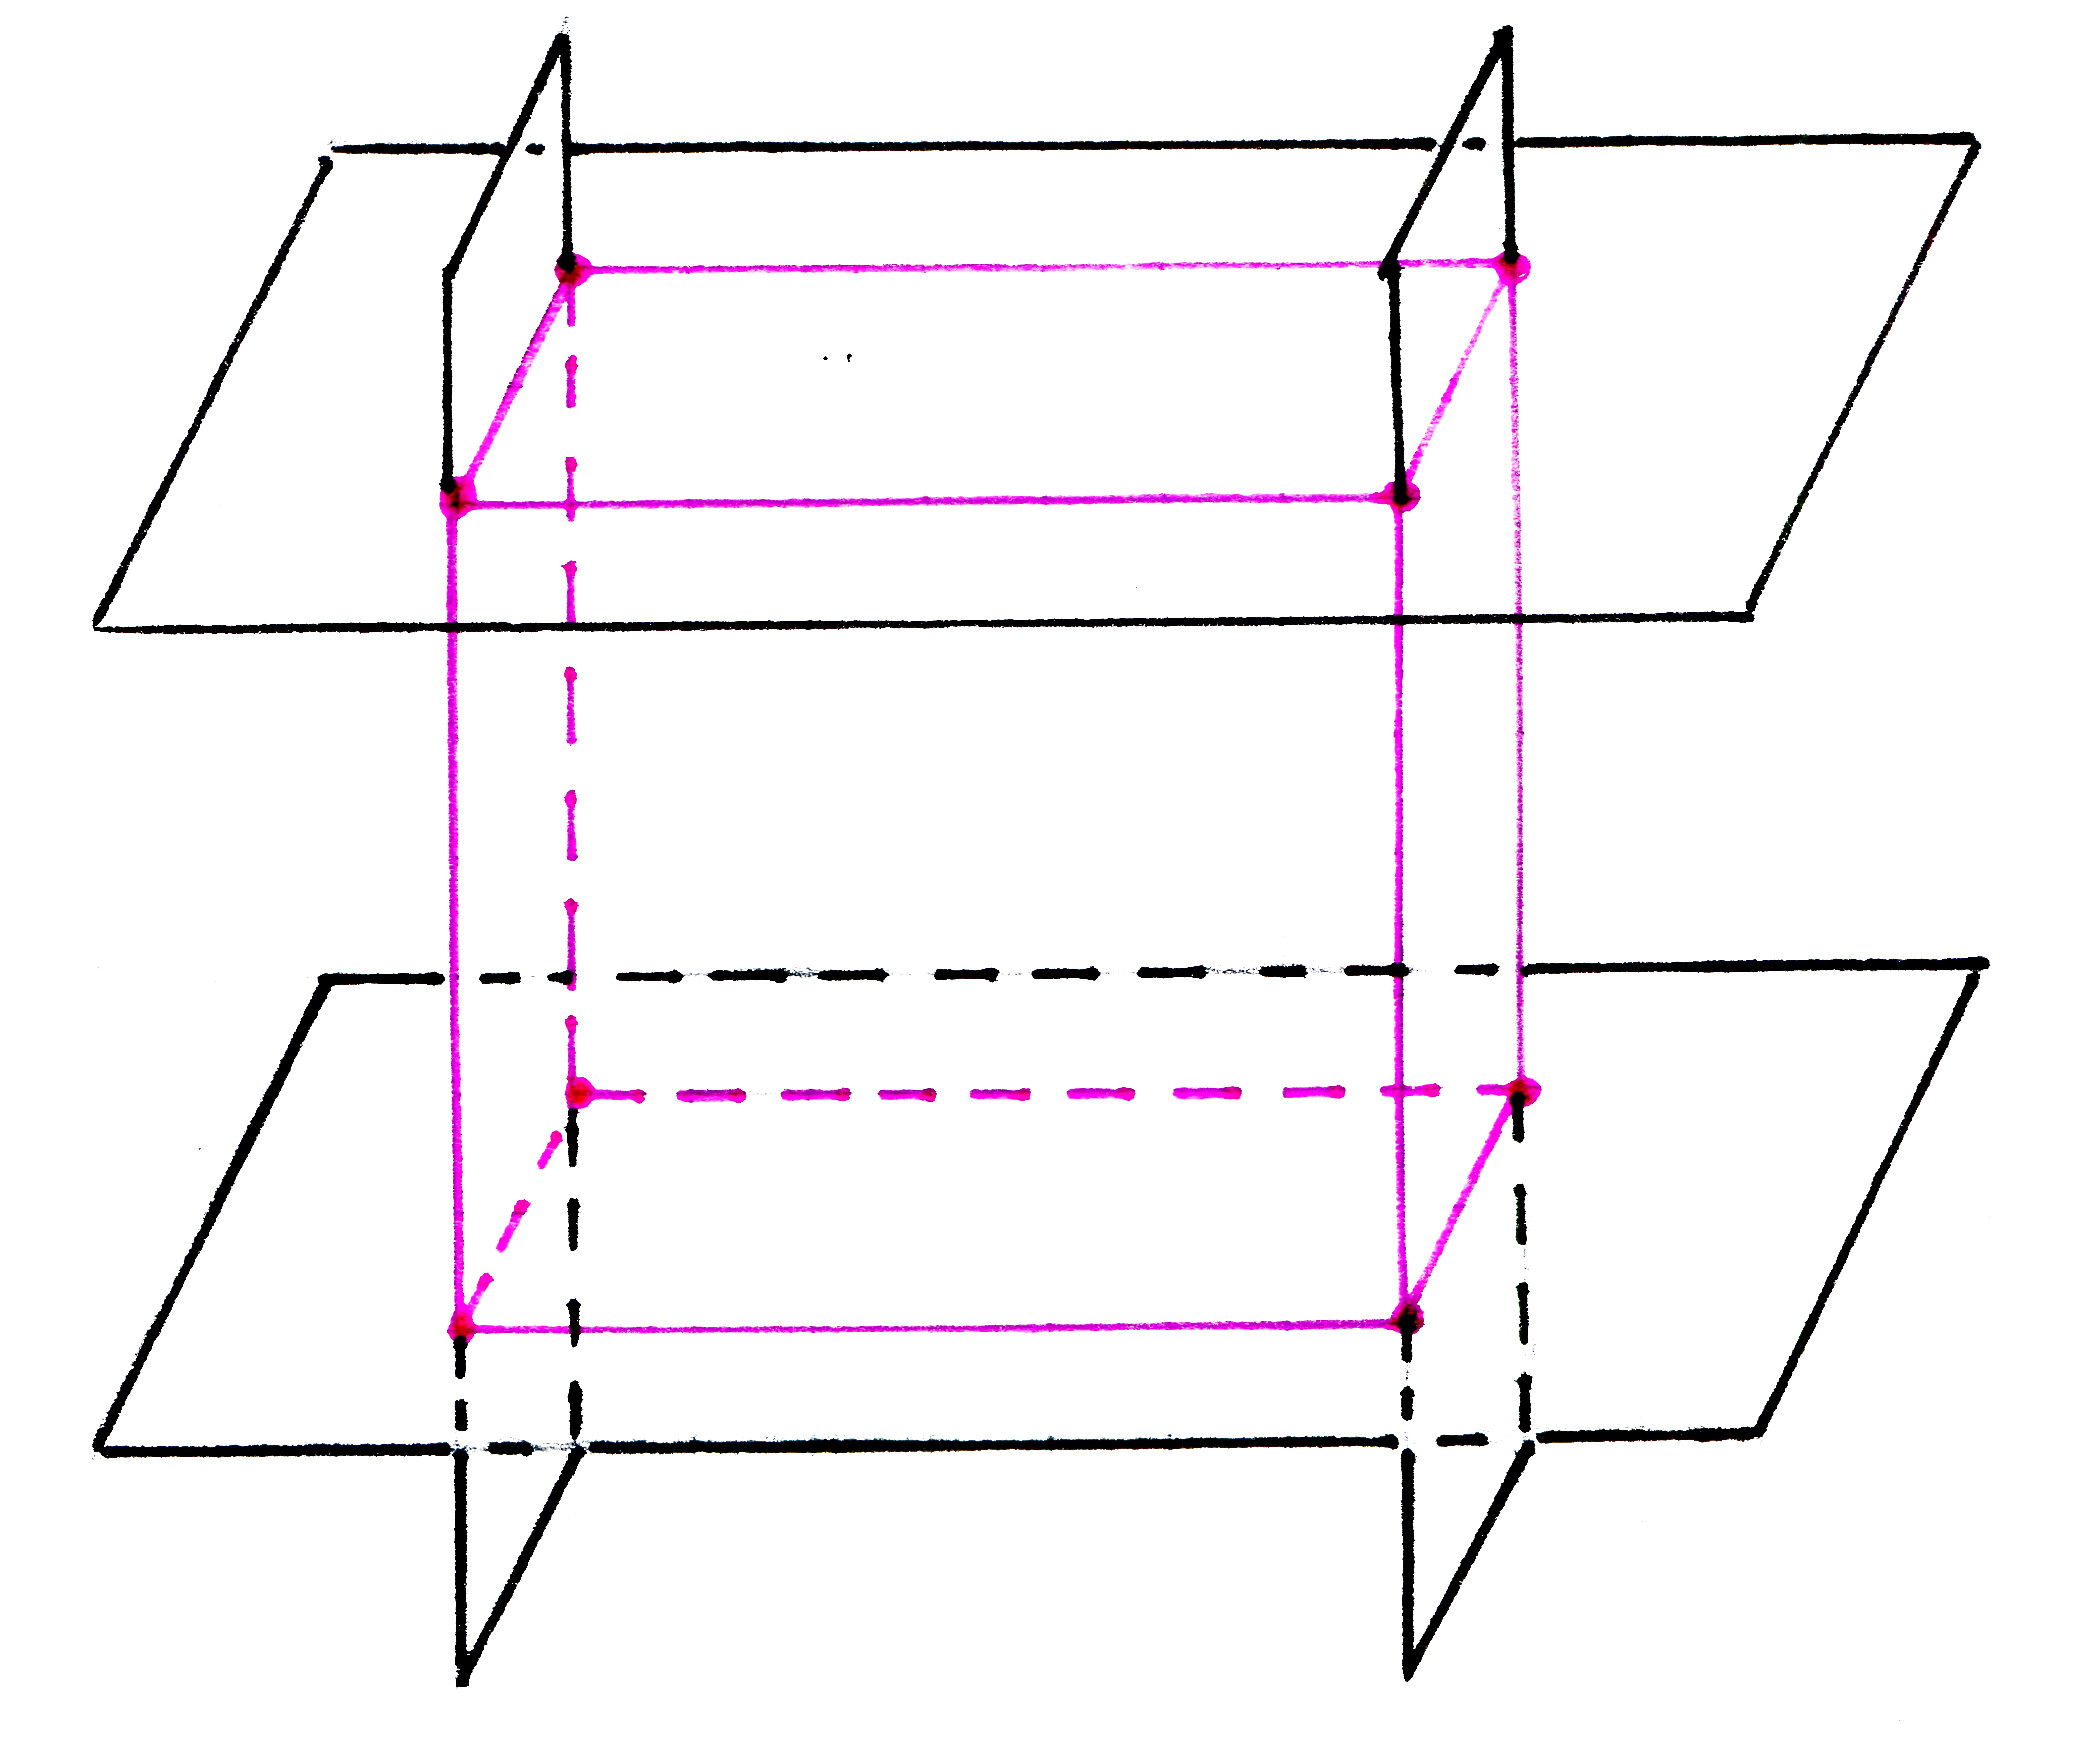
\includegraphics[width=.8\textwidth]{VollerWuerfel}
      \caption{Ein voller Würfel, beschränkt durch seine Seitenflächen. Vorder- und Rückseite sind zur Übersichtlichkeit weggelassen}
    \end{figure}
  \end{minipage}
\end{definition}

\begin{remark}[Bezug von Polyedern zu Graphen]
  Das \term{1-Skelett}\label{def:skelett} von \( P \) (also die Menge der Ecken und Kanten) von \( P \) ist ein Graph in \( \R^3 \). \\
  Man kann zeigen (Resultat der konvexen Geometrie): durch Zentralprojektion von einem Punkt nahe bei einem ``Seitenmittelpunkt'' auf eine geeignete Ebene wird das \( 1 \)-Skelett \( p^{(1)} \) von \( P \) auf einen \emph{ebenen} Graphen \( G_p \) abgebildet (sog. \term{Schlegel-Diagramm}\label{def:schlegelDiagramm}). Es gilt dann: \( s(P) = s(G_p) \), \( k(P) = k(G_p) \), \( e(P) = e(G_p) \).
  \begin{figure}[H]
    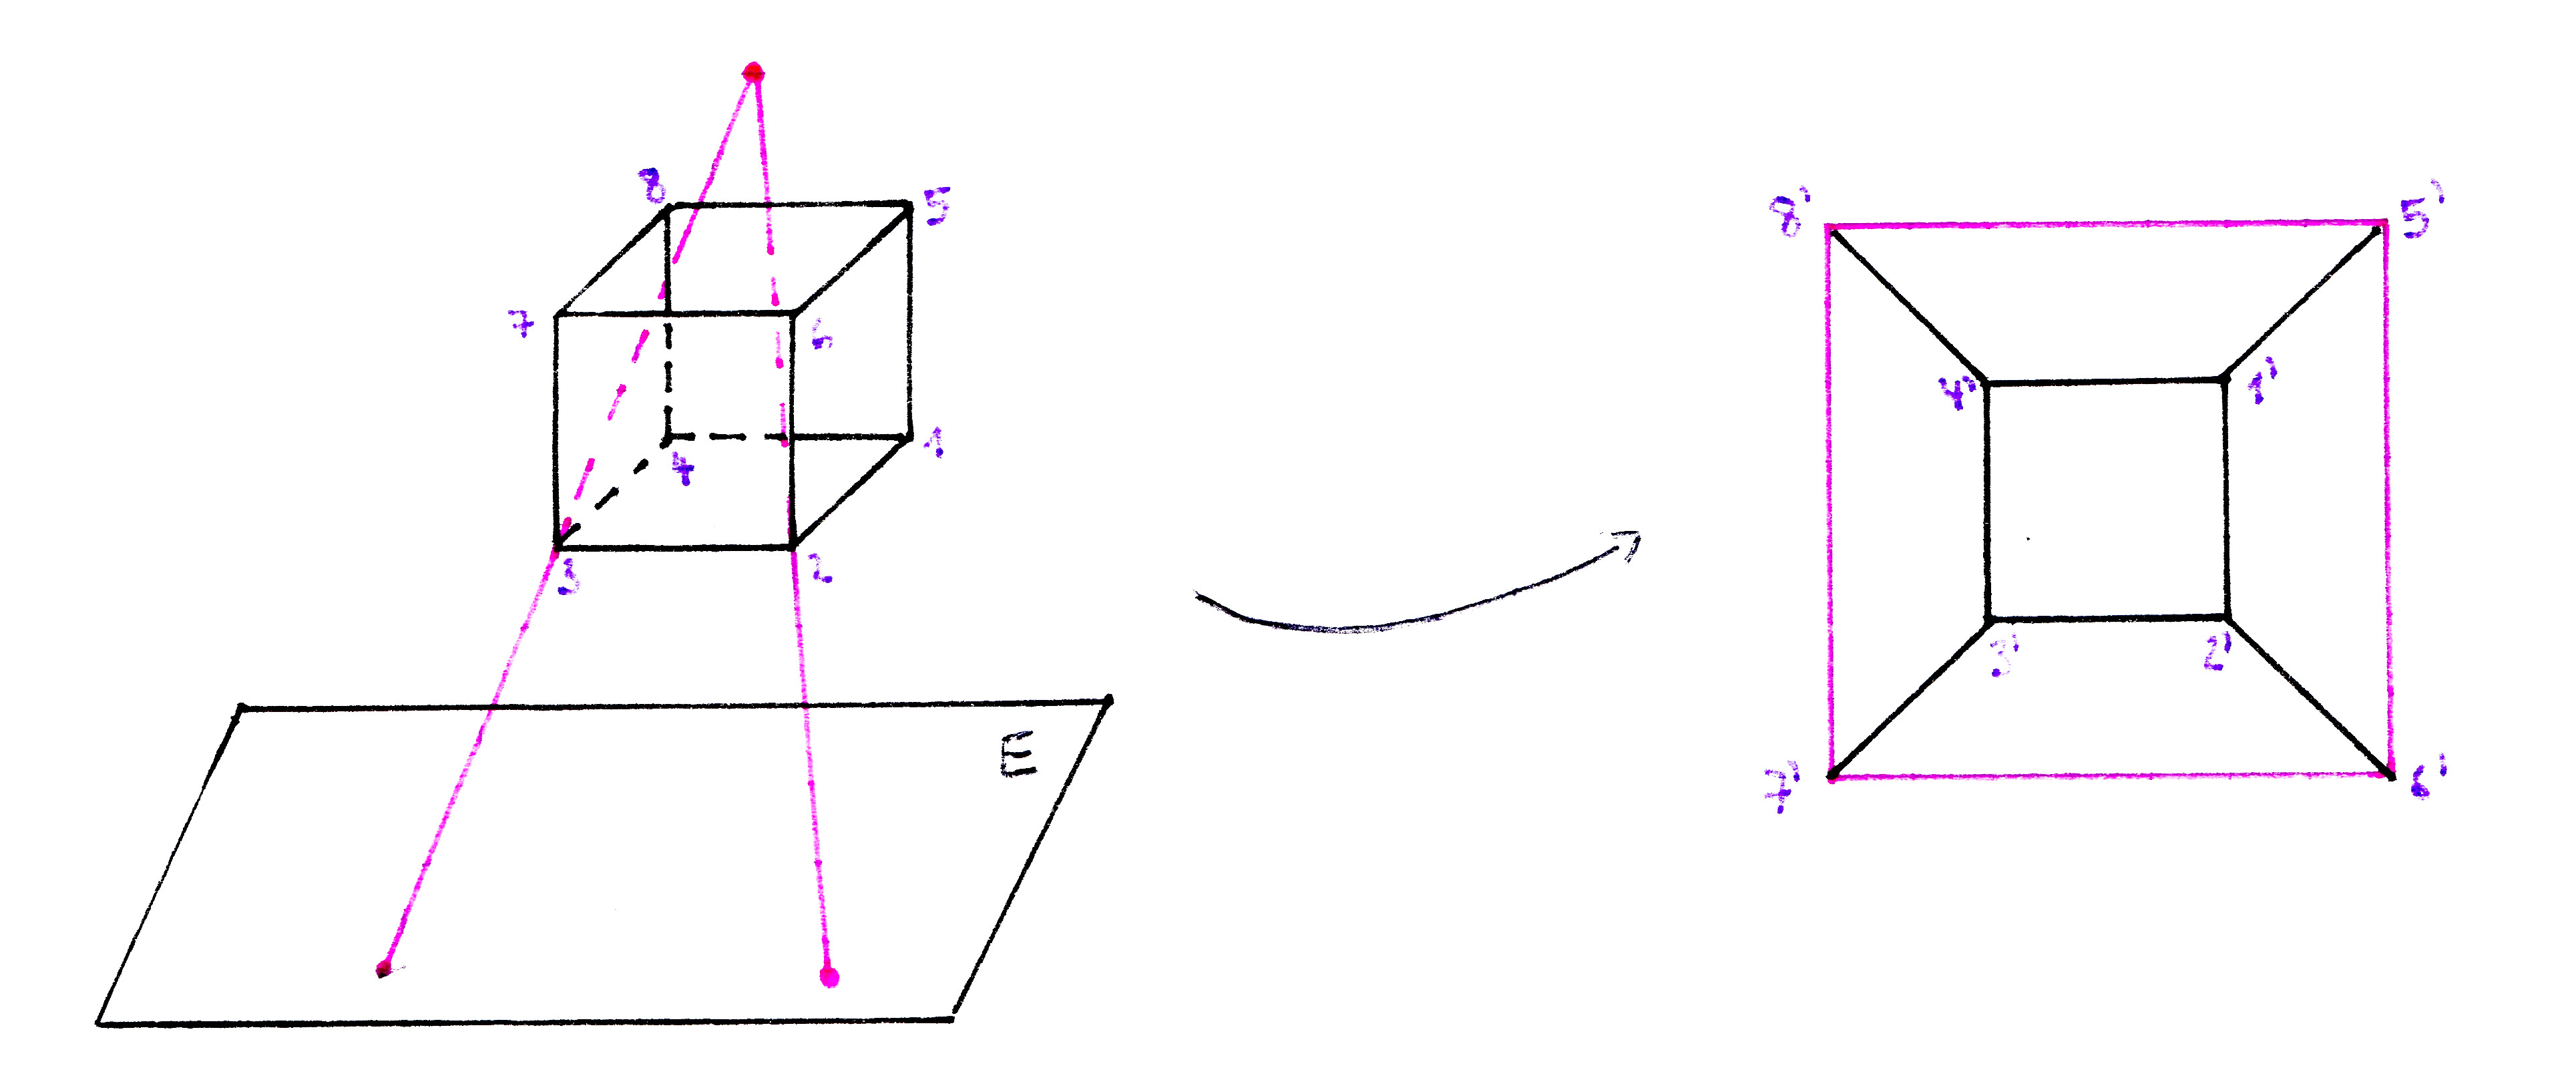
\includegraphics[width=.8\textwidth]{VollerWuerfelEbene}
    \caption{Projektion des vollen Würfels auf die Ebene}
  \end{figure}
\end{remark}

\begin{deduction}[Eulersche Polyeder-Formel]
  \begin{equation*}
    e(P) - k(P) + s(P) = 2\text{.}
  \end{equation*}
\end{deduction}

\begin{definition}[Regulärer Polyeder]
  Ein Polyeder in \( \R^3 \) heißt \term{regulär}\label{def:regulaererPolyeder}, falls alle Seitenflächen kongruente reguläre \( n \)-Ecke (also haben sie gleich lange Kanten) sind und in jeder Ecke \( m \) solche \( n \)-Ecke zusammentreffen (insbesondere gehen von jeder Ecke \( m \) Kanten aus).
\end{definition}

\begin{theorem}[Platonische Körper]
  Es gibt genau \( 5 \) reguläre Polyeder in \( \R^3 \):
  \begin{align*}
    (m,n) &= (3,3) \quad \text{Tetraeder}  \\
     &= (3,4) \quad \text{Würfel} \\
     &= (4,3) \quad \text{Oktaeder} \\
     &= (3,5) \quad \text{Dodekaeder} \\
     &= (5,3) \quad \text{Ikosaeder}
  \end{align*}
  \begin{proof}
    \
    \begin{itemize}
      \item \textbf{Existenz}: Explizite Konstruktion, siehe Euklid (oder Tutorium (oder basteln (oder Google))).
      \item \textbf{Vollständigkeit}: Sei \( s = \) Anzahl an Seitenflächen. Dann gilt: \( s*n = 2k \), ebenso \( m*e = 2k \) und damit
        \begin{equation*}
          n*s = 2k = m*e \Rightarrow k = \frac{me}{2} \quad s = \frac{me}{n}
        \end{equation*}
        Euler-Polyeder-Formel für \( P \) beziehungsweise \( G_p \) ergibt:
        \begin{equation*}
          2 = e-k+s = e - \frac{me}{2} + \frac{me}{n} \Leftrightarrow 4n = e\left( 2n - nm + 2m \right)\text{.}
        \end{equation*}
        Da \( n > 0 \) und \( e > 0 \) folgt:
        \begin{equation*}
          2n - nm + 2m > 0 \Leftrightarrow nm - 2n - 2m + 4 < 4 \Leftrightarrow (n-2)(m-2) < 4\text{.}
        \end{equation*}
        Man sieht, dass es nur obenstehende Möglichkeiten gibt. \qed{}
    \end{itemize}
  \end{proof}
\end{theorem}

\begin{definition}[Euler-Charakteristik von Simplizialkomplexen]
  Sei \( K \) ein Simplizialkomplex. Dann ist die \term{Euler-Charakteristik}\label{def:eulercharakteristikSimplizialkomplex} von \( K \):
  \begin{equation*}
    \chi(K) \coloneqq \alpha_0-\alpha_1+\alpha_2 \mp \dots \pm \alpha_k = \sum_{i = 0}^k {(-1)}^i\alpha_i\text{,}
  \end{equation*}
  wobei \( \alpha_i = \) Anzahl von \( i \)-Simplices in \( K \). \\
  Die sogenannten ``\term{Betti-Zahlen}''\label{def:bettiZahlen} lassen sich berechnen mit Methoden aus der algebraischen Topologie (als Dimension von gewissen Vektorräumen, die man zu \( K \) konstruiert). \\
  Man zeigt: \( \chi(K) \) ist eine topologische Invariante, also 
  \begin{equation*}
    \vert K \vert \underset{\text{homö}}{\cong} \vert \widetilde{K} \vert \Rightarrow \chi(K) = \chi(\widetilde{K})\text{.}
  \end{equation*}
  Ein topologischer Raum \( X \) heißt \term{triangulierbar}\label{def:triangulierbar}, falls ein (endlicher) Simplizialkomplex \( K \) existiert und ein Homöomorphismus \( \vert K \vert \overset{\sim}{\to} X \). \\
  Ist \( X \) (via \( K \)) triangulierbar, so definiert man \( \chi(X) \coloneqq \chi(K) \) (und zeigt, dass \( \chi(X) \) unabhängig von der gewählten Triangulierung ist). \\
  Nun ist \( \chi(S^2) = \chi(\text{Tetraeder}) = 2 \) und jeder (reguläre) Polyeder homöomorph zu \( S^2 \), also \( \chi(P) = \chi(S^2) = 2 \).
\end{definition}

\section{Spezielle Konstruktion von Quotientenräumen (``Verkleben'')}

\begin{definition}[Verklebung]
  \( X \) und \( Y \) seien topologische Räume, \( A \subset X \) ein Teilraum und \( f: A \to Y \) eine Abbildung (nicht notwendigerweise stetig). Sei \( X \cupdot Y \) die disjunkte Vereinigung. Definiere eine Äquivalenzrelation auf \( X \cupdot Y \) via \( f \) wie folgt:
  \begin{equation*}
    x \sim x' \overset{\text{Def}}{\Leftrightarrow} \begin{cases}
      &x = x' \\
      \text{oder } &f(x) = x' \quad (x \in A) \\
      \text{oder } &f(x') = x \quad (x' \in A) \\
      \text{oder } &f(x) = f(x') \quad (x, x' \in A)
    \end{cases}
  \end{equation*}
  Das ist eine Äquivalenzrelation. \\
  Der Quotientenraum \( X \cup_f Y \coloneqq X \cupdot Y /_\sim \) heißt \term{Verklebung}\label{def:verklebung} von \( Y \) an \( Y \) via \( f \).
\end{definition}

\begin{example} \
  \begin{enumerate}
    \item \( X = Y = S^1 \), \( A = \{ x_0 \} \), \( f(x_0) \coloneqq x_0 \)
      \begin{figure}[H]
        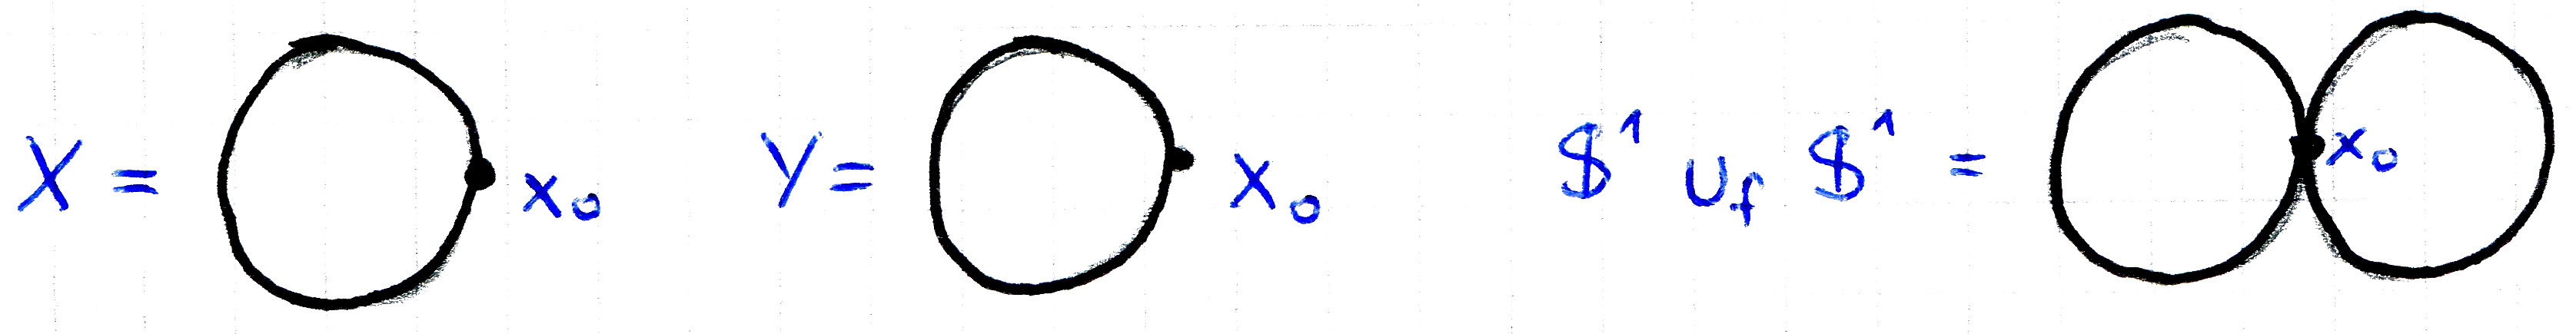
\includegraphics[width=.5\textwidth]{EinfacheVerklebung}
        \caption{Einfache Verklebung}
      \end{figure}
    \item \( X = [0,1] \), \( Y = [2,5] \), \( A = \{ 0,1 \} \subset X \), \( f(0) = 2 \), \( f(1) = 3 \)
    \begin{figure}[H]
      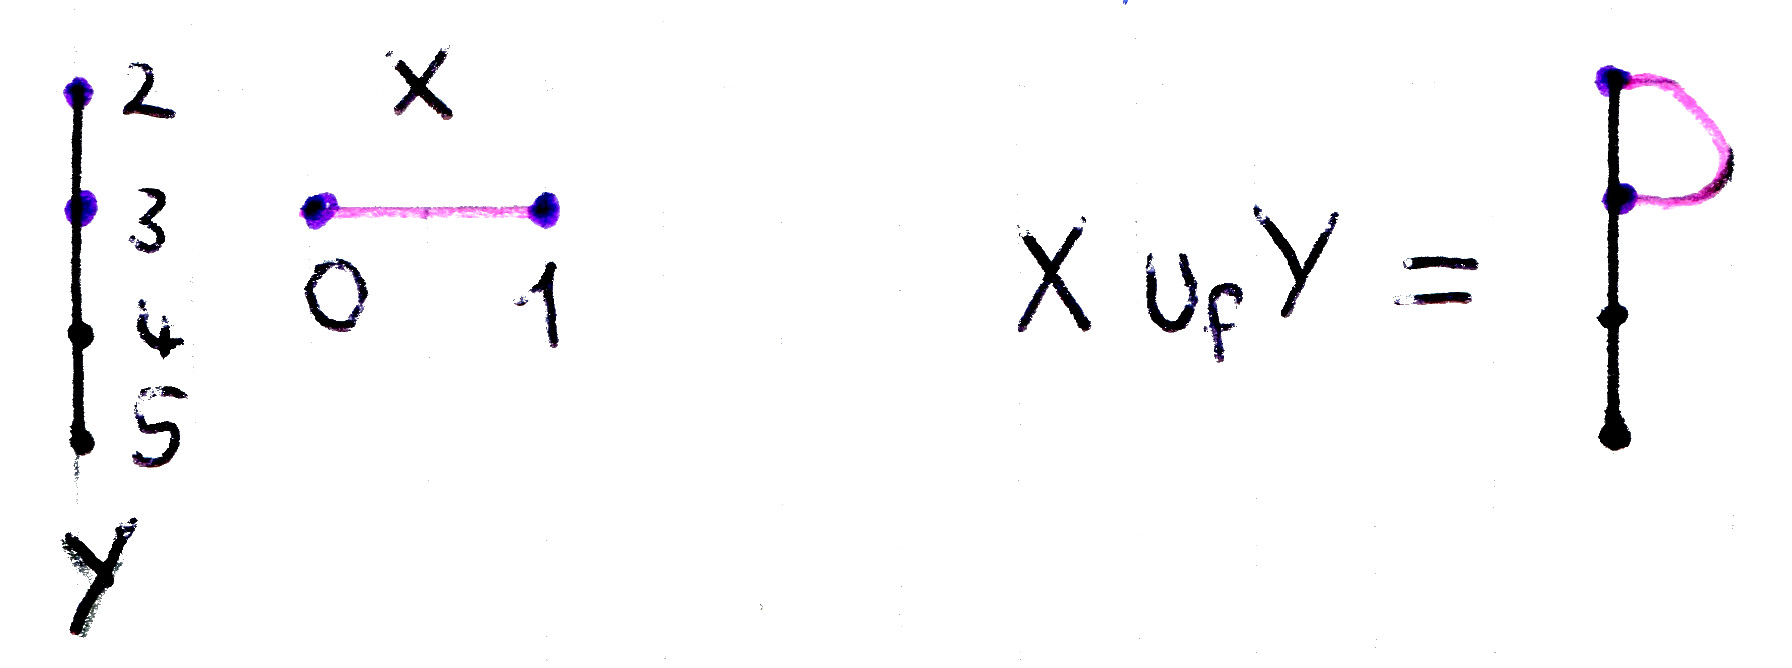
\includegraphics[width=.5\textwidth]{Intervallverklebung}
      \caption{Intervallverklebung}
    \end{figure}
    \item \emph{Zusammenhängende Summe} von \( 2 \)-Mannigfaltigkeiten \( M_1 \) und \( M_2 \).
      \begin{figure}[H]
        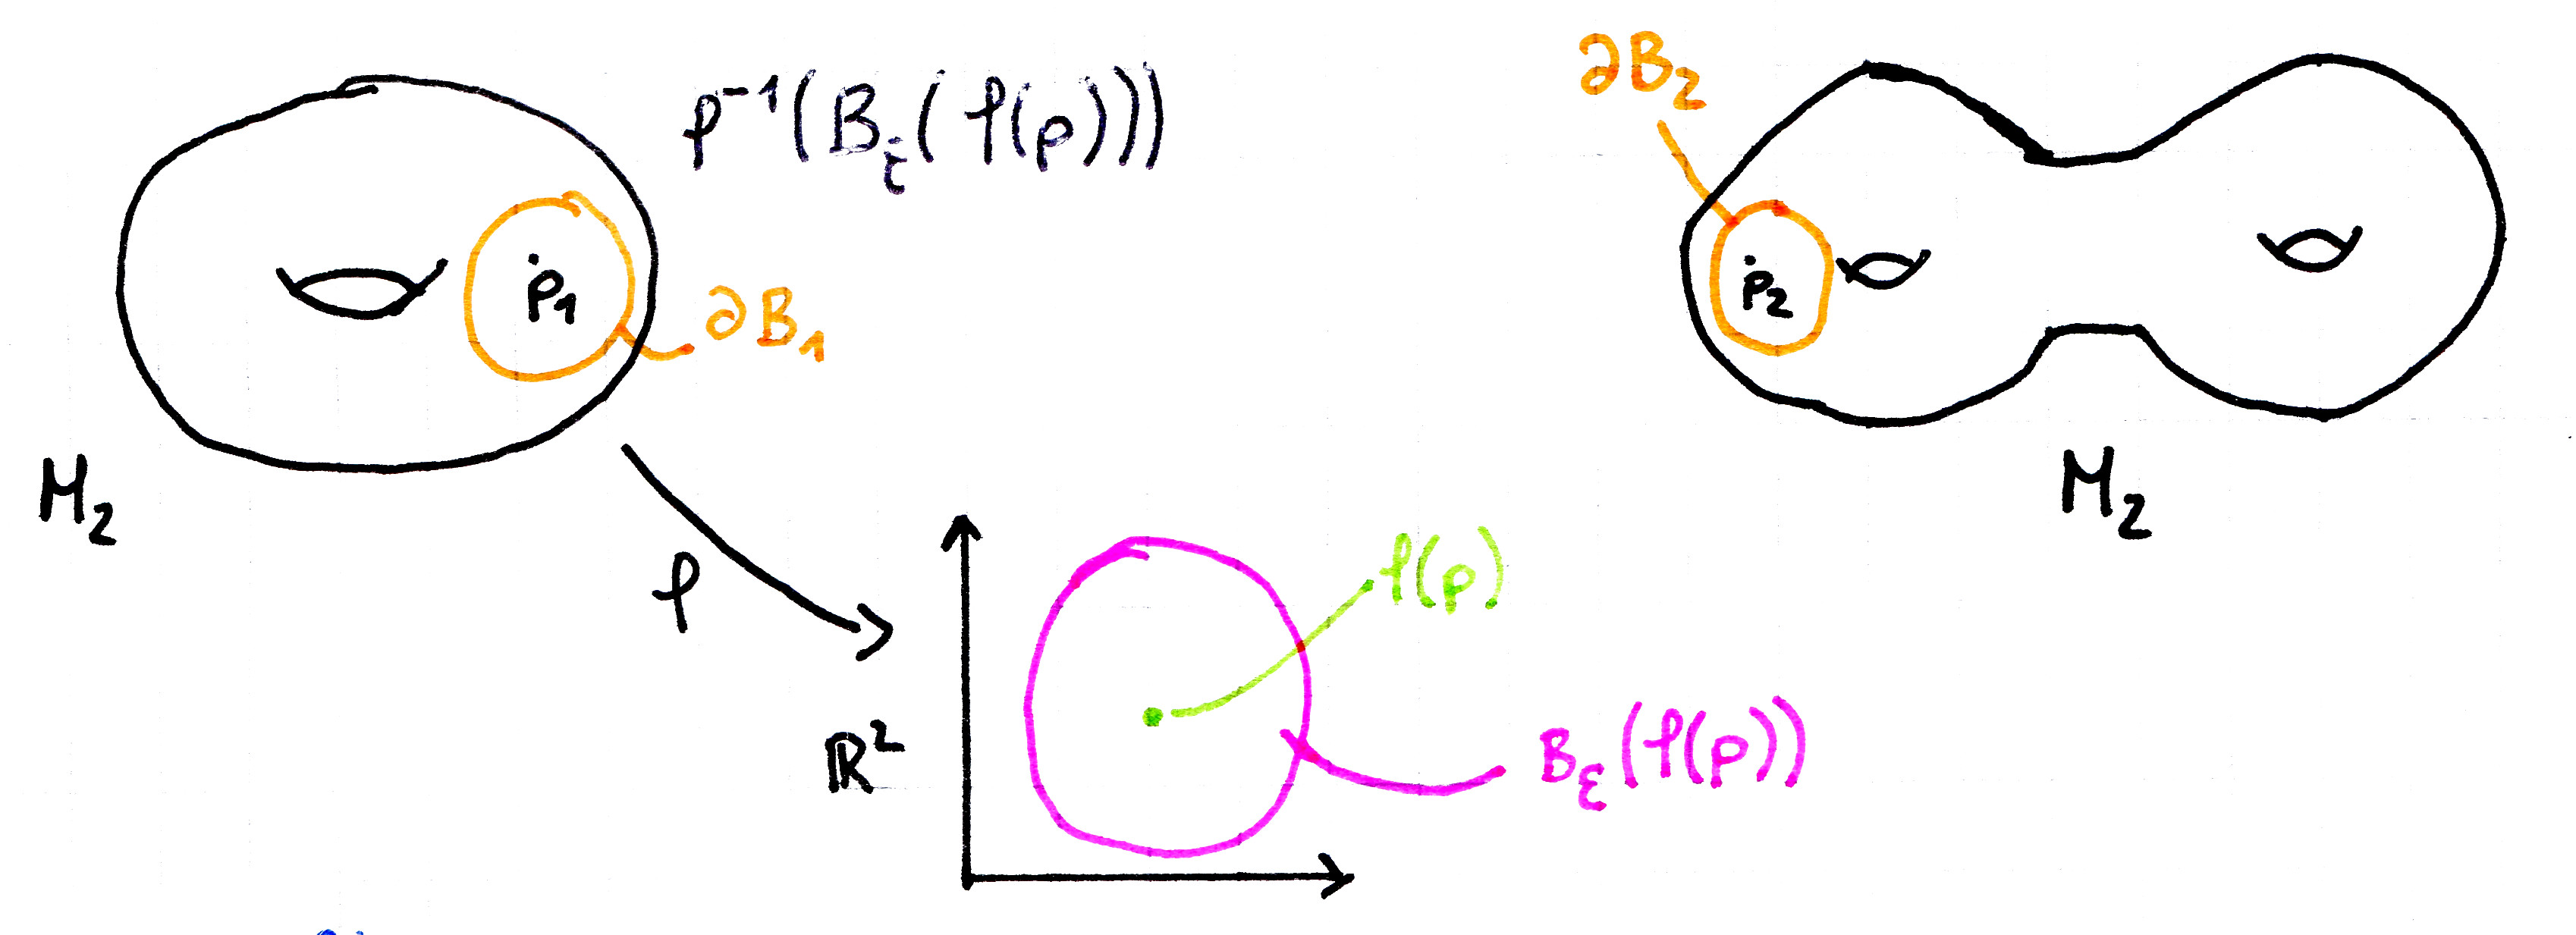
\includegraphics[width=.8\textwidth]{ZusammenhaengendeSumme}
        \caption{Zusammenhängende Summe von \( 2 \)-Mannigfaltigkeiten}
      \end{figure}
      Konstruktion:
      \begin{enumerate}
        \item Entferne geeignet kleine abgeschlossene ``Kreisscheiben'' von \( p_1 \in M_1 \) und \( p_2 \in M_2 \) mit Rändern \( \delta B_1 \) und \( \delta B_2 \) Homöomorph zu \( S^1 \).
        \item Wähle Homöomorphismus \( f: \delta B_1 \to \delta B_2 \).
        \item Verklebe \( M_1 \) und \( M_2 \) mittels \( f : M_1 \cup_f M_2 \eqqcolon M_1 \# M_2 \)
        \begin{figure}[H]
          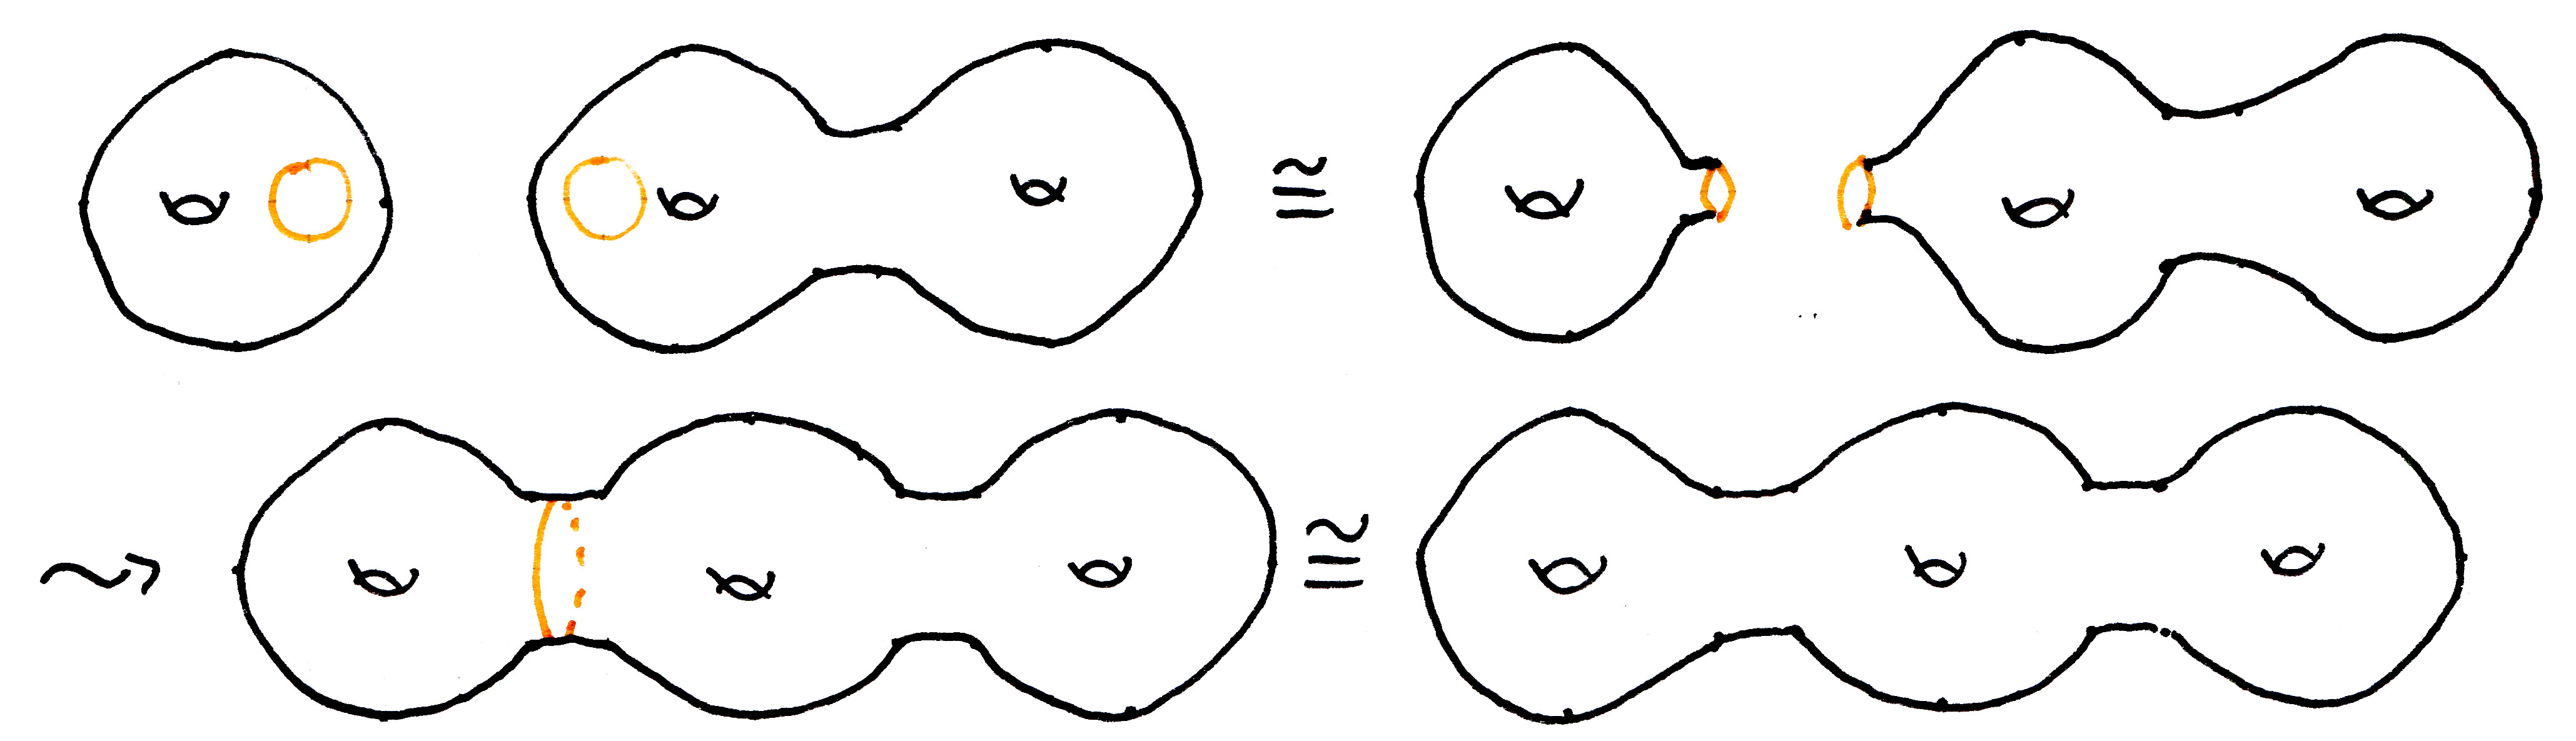
\includegraphics[width=.8\textwidth]{Verklebung}
          \caption{Verklebung}
        \end{figure}
      \end{enumerate}
      Alle kompakten geschlossenen Flächen kann man aus \( S^2 \) konstruieren durch Verkleben Tori.
      \begin{figure}[H]
        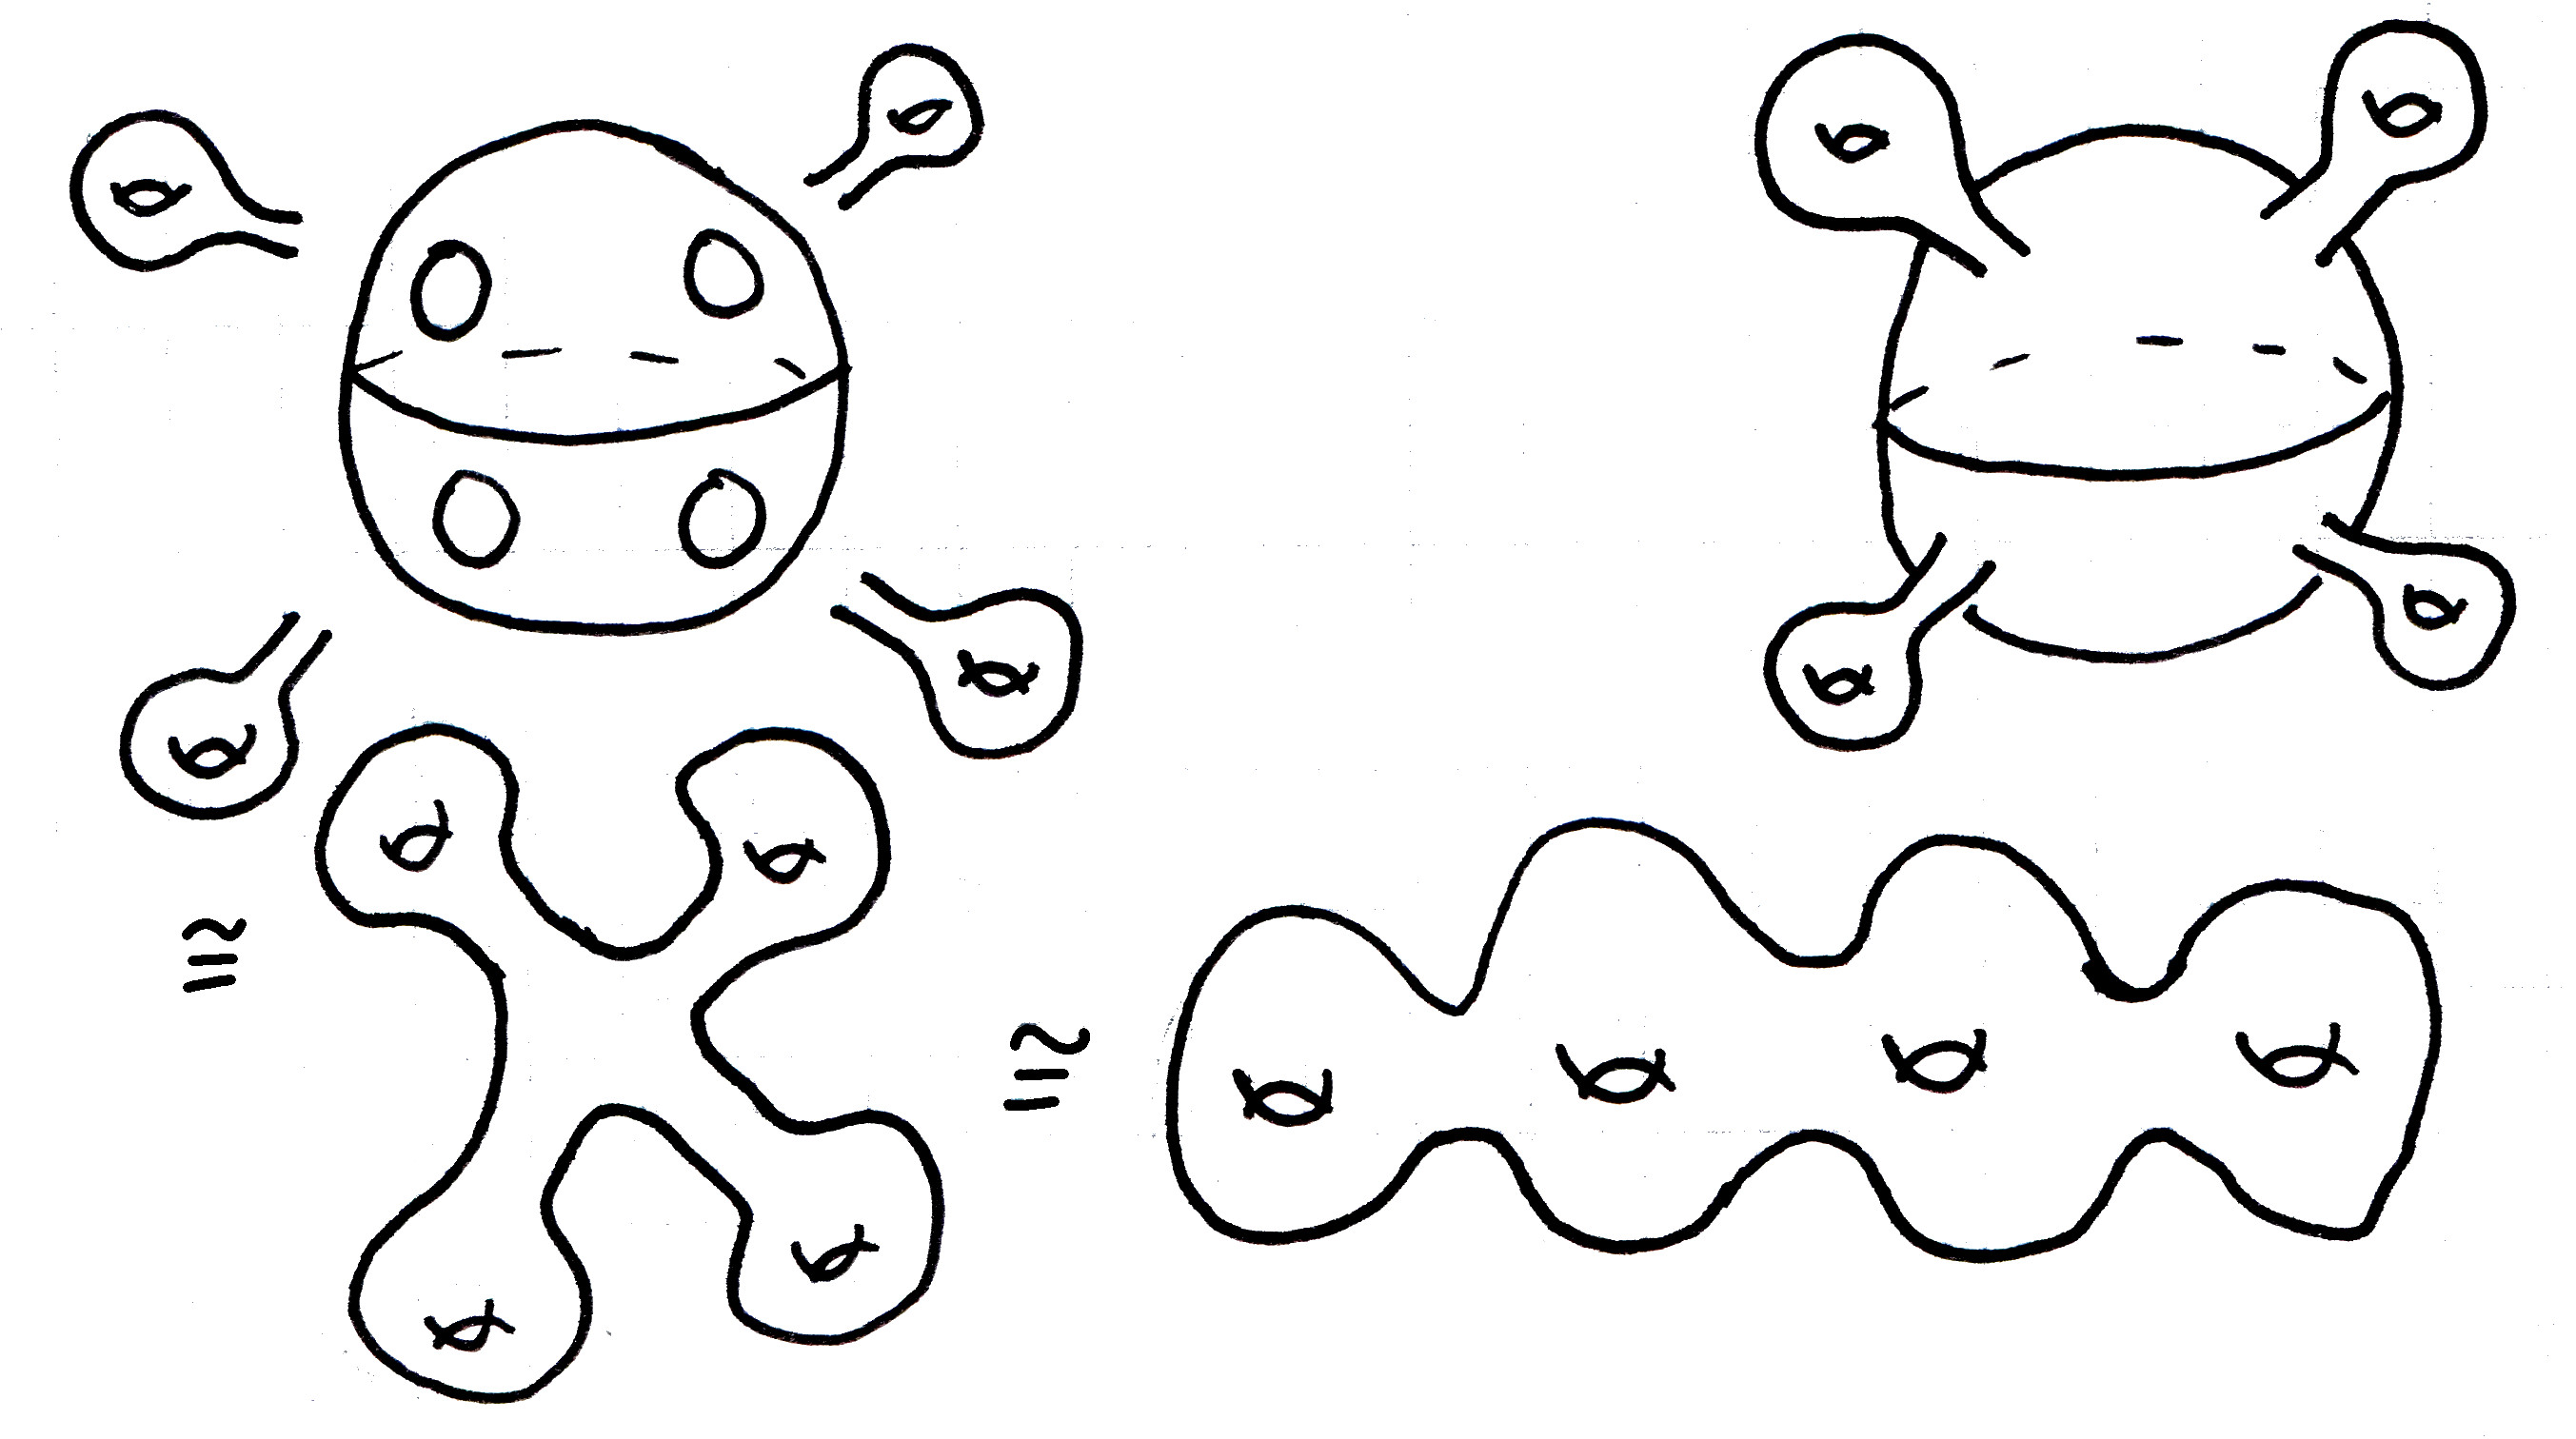
\includegraphics[width=.5\textwidth]{BeliebigeGeschlosseneFlaeche}
        \caption{Konstruieren einer beliebigen kompakten geschlossenen Fläche aus \( S^2 \)}
      \end{figure}
  \end{enumerate}
\end{example}

\begin{remark}[Selbstverklebungen]
  ``\term{Selbst-Verklebungen}''\label{def:selbstverklebung} sind analog definiert: \\
  \( X = \) topologischer Raum, \( A \subset X \) Teilraum, \( f : A \to X \), \( X_f \coloneqq X/_\sim \) mit Äquivalenzrelation wie oben.
\end{remark}

\begin{example}
  \
  \begin{enumerate}
    \item \( X = [0,1] \times [0,1] \) = Einheitsquadrat,

      \begin{minipage}{.45\textwidth}
        \begin{align*}
          A \subset \delta X = &\underbrace{\left( \{ 0 \} \times [0,1] \right)}_{\eqqcolon A_1} \cup \underbrace{\left( \{ 1 \} \times [0,1] \right)}_{\eqqcolon B_2} \\
          &\cup \underbrace{\left( [0,1] \times \{ 0 \} \right)}_{\eqqcolon A_2} \cup \underbrace{\left( [0,1] \times \{ 1 \} \right)}_{\eqqcolon B_2}\text{,}
        \end{align*}
      \end{minipage}
      \hfill
      \begin{minipage}{.45\textwidth}
        \begin{figure}[H]
          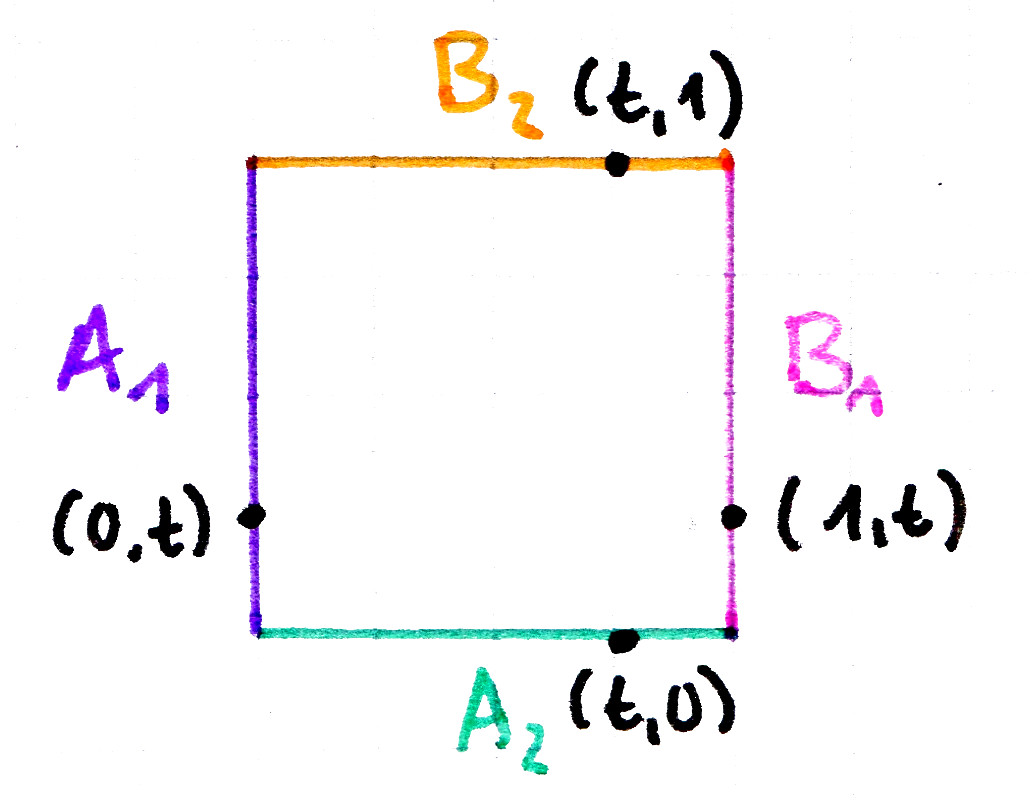
\includegraphics[width=.8\textwidth]{VorbereitungVerklebungEinheitsquadrat}
          \caption{Vorbereitung zur Selbstverklebung am Einheitsquadrat}
        \end{figure}
      \end{minipage}

      \( A \coloneqq A_1 \cup A_2 \),
      \begin{align*}
        f: &A_1 \to B_1, \quad (0,t) \mapsto (1,t) \\
         &A_2 \to B_2, \quad (t,0) \mapsto (t,1)
      \end{align*}
      \begin{figure}[H]
        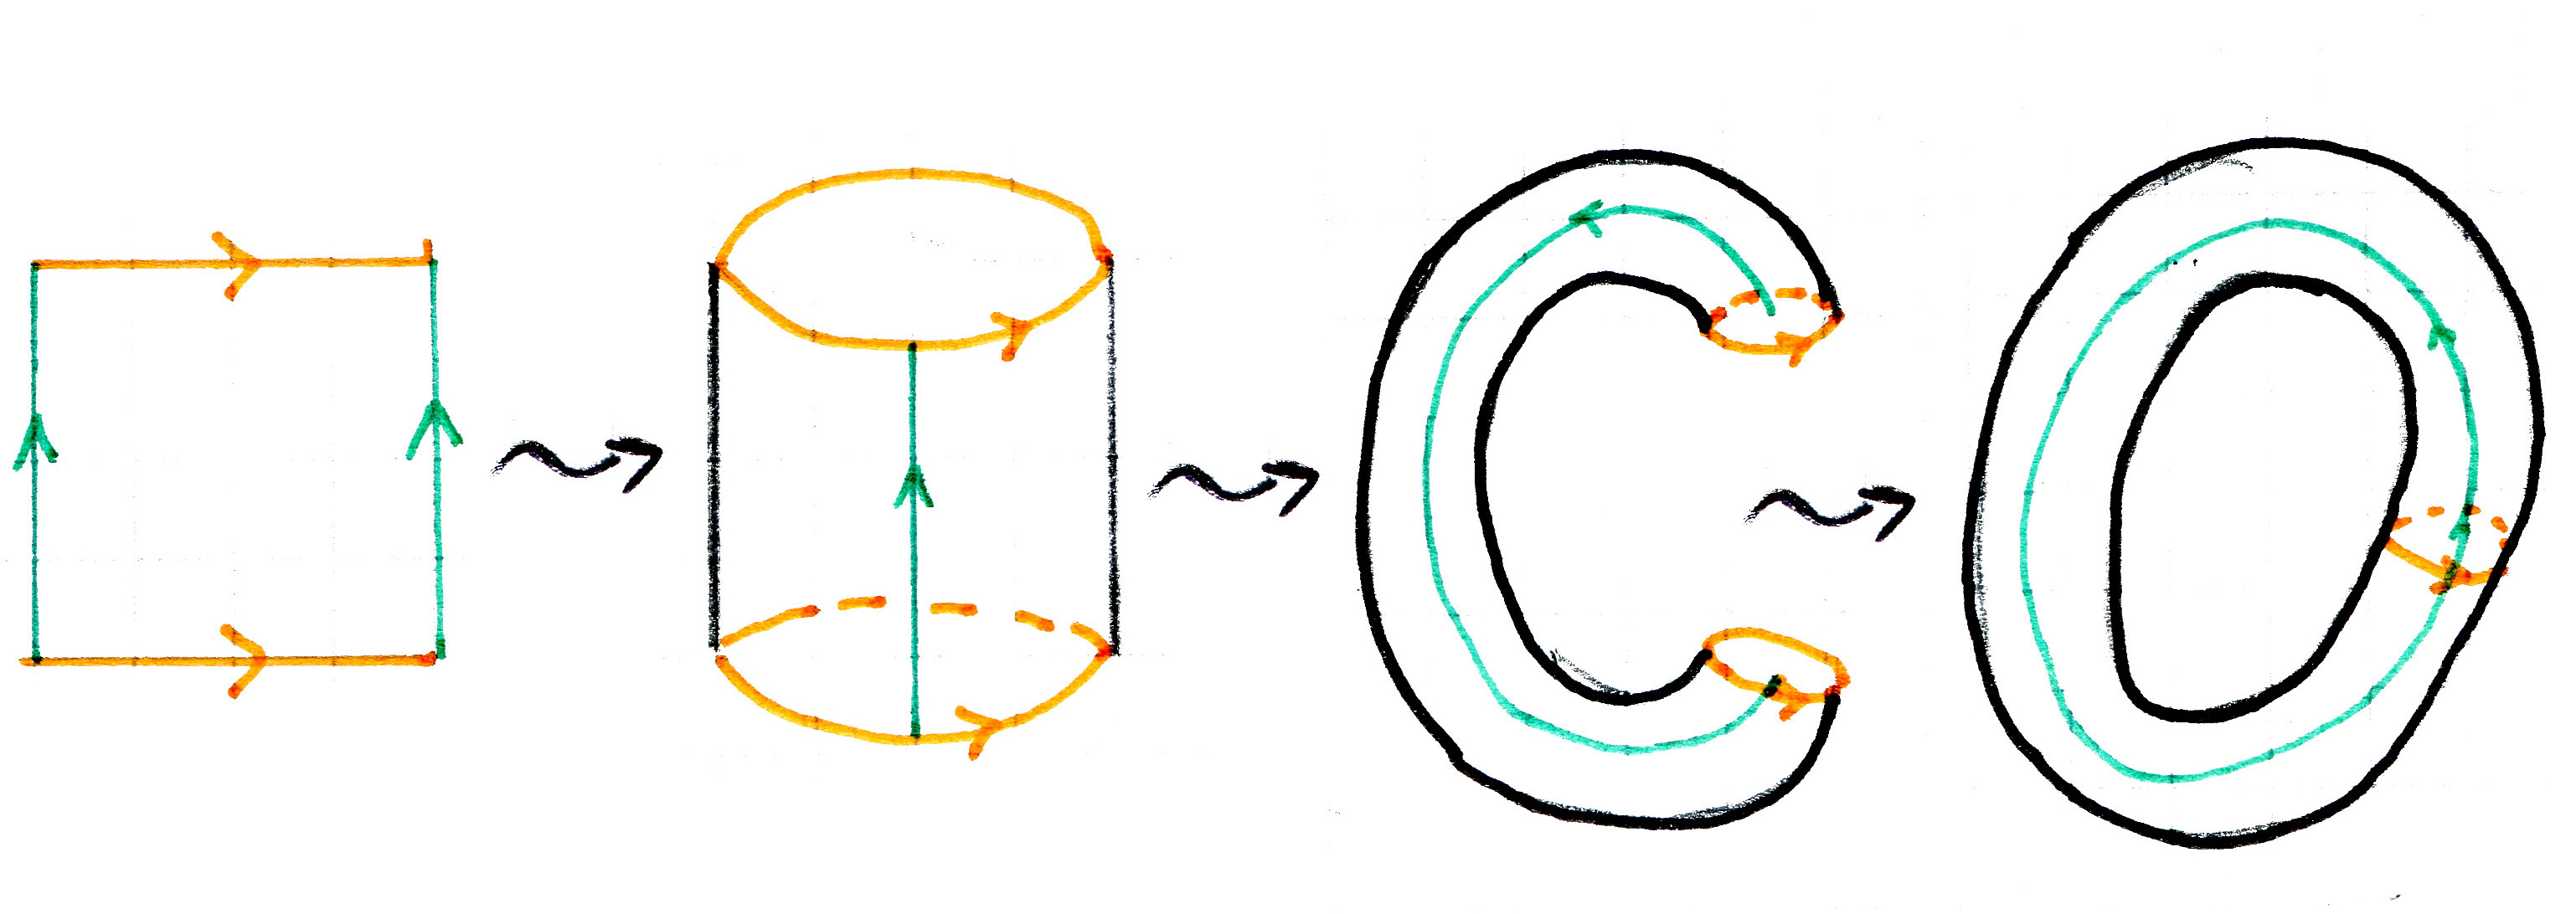
\includegraphics[width=.8\textwidth]{Verklebungsprozess}
        \caption{Verklebungsprozess}
      \end{figure}
    \item \emph{Möbiusband}: \( X = [0,1] \times [0,1] \), \( A = A_1 \), \( f: A_1 \ni (0,1) \mapsto (1,1-t) \in B_1 \)
    % TODO BSP7
    \item \emph{Projektive Ebene}: \( P^2\R \) entsteht durch Verkleben einer Kreisscheibe und eines Möbiusbandes längs der Ränder.
    % TODO BSP8
    % TODO BSP9 --- Kleinsche Flasche
  \end{enumerate}
\end{example}
